\documentclass[%
%%% PARA ESCOLHER O ESTILO TIRE O SIMBOLO %(COMENTÁRIO)
%SemVinculoColorido,
%SemFormatacaoCapitulo,
%SemFolhaAprovacao,
%SemImagens,
%CitacaoNumerica, %% o padrão é citação tipo autor-data
PublicacaoDissOuTese, %% (é também o "default") com ficha catal. e folha de aprovação em branco. Caso tenha lista de símbolos e lista de siglas e abreviaturas retirar os comentários dos arquivos siglas.tex e abreviaturasesiglas.tex. Retirar também os comentários indicados nesse arquivo, nos includes
%PublicacaoArtigoOuRelatorio, %% texto sequencial, sem quebra de páginas nem folhas em branco
%PublicacaoProposta, %% igual tese/dissertação, mas sem ficha catal. e fol. de aprov.
%PublicacaoLivro, %% com capítulos
%PublicacaoLivro,SemFormatacaoCapitulo, %% sem capítulos
english,portuguese %% para os documentos em Português com abstract.tex em Inglês
%portuguese,english %% para os documentos em Inglês com abstract.tex em Português
,LogoINPE% comentar essa linha para fazer aparecer o logo do Governo
,CCBYNC	% as opções de licença são: CCBY, CCBYSA, CCBYND, CCBYNC, CCBYNCSA, CCBYNCND, GPLv3 e INPECopyright
]{tdiinpe}
%]{../../../../../iconet.com.br/banon/2008/03.25.01.19/doc/tdiinpe}

% PARA EXIBIR EM ARIAL TIRAR O COMENTÁRIO DAS DUAS LINHAS SEGUINTES
%\renewcommand{\rmdefault}{phv} % Arial
%\renewcommand{\sfdefault}{phv} % Arial

% PARA PUBLICAÇÕES EM INGLÊS:
% renomear o arquivo: abnt-alf.bst para abnt-alfportuguese.bst
% renomear o arquivo: abnt-alfenglish.bst para abnt-alf.bst


%%%%%%%%%%%%%%%%%%%%%%%%%%%%%%%%%%%%%%%%%%%%%
%%% Pacotes já previamente carregados:      %
%%%%%%%%%%%%%%%%%%%%%%%%%%%%%%%%%%%%%%%%%%%%%%%%%%%%%%%%%%%%%%%%%%%%%%%%
%%% ifthen,calc,graphicx,color,inputenc,babel,hyphenat,array,setspace, %
%%% bigdelim,multirow,supertabular,tabularx,longtable,lastpage,lscape, %
%%% rotate,caption2,amsmath,amssymb,amsthm,subfigure,tocloft,makeidx,  %
%%% eso-pic,calligra,hyperref,ae,fontenc                               %
%%%%%%%%%%%%%%%%%%%%%%%%%%%%%%%%%%%%%%%%%%%%%%%%%%%%%%%%%%%%%%%%%%%%%%%%
%%% insira neste campo, comandos de LaTeX %%%
%%% \usepackage{_exemplo_}
% etc.
%%%%%%%%%%%%%%%%%%%%%%%%%%%%%%%%%%%%%%%%%%%%%

%\watermark{No. 0.1} %% use o comando \watermark para identificar a versão de seu documento
%% comente este comando quando for gerar a versão final
\usepackage{rotating}
\usepackage{dsfont}
\usepackage{comment}

%%%%%%%%%%%%%%%%%%%CAPA%%%%%%%%%%%%%%%%%%%%%%%%%%%%%%%%
%\serieinpe{INPE-NNNNN-TDI/NNNN} %% não mais usado

\titulo{Escrever o título no idioma em que foi escrito a publicação}
\title{Escrever o título em Inglês para publicações escritas em Português e em Português para publicações escritas em Inglês} %% 
\author{Nome Completo do Autor1\\Nome Completo do Autor2} %% coloque o nome do(s) autor(es)
\descriccao{Tese de Doutorado ou Dissertação de Mestrado do Curso de Pós-Graduação em Nome do Curso, orientada pelo(a) Dr(a). Nome do Orientador(a), aprovada em dd de mês por extenso de aaaa.}
\repositorio{aa/bb/cc/dd} %% repositório onde está depositado este documento - na omissão, será preenchido pelo SID
\tipoDaPublicacao{TDI}	%% tipo da publicação (NTC, RPQ, PRP, MAN, PUD, TDI, TAE e PRE) na ausência do número de série INPE, caso contrário deixar vazio
\IBI{xx/yy} %% IBI (exemplo: J8LNKAN8PW/36CT2G2) quando existir, caso contrário o nome do repositório onde está depositado o documento

\date{AAAA}%ano da publicação

%%%%%%%%%%%%%%%%%%%%%%%%%%VERSO DA CAPA%%%%%%%%%%%%%%%%%%%%%%%%%%%%%%%%%%%%%%%%%%%%%%%
\tituloverso{\vspace{-0.9cm}\textbf{\PublicadoPor:}}
\descriccaoverso{Instituto Nacional de Pesquisas Espaciais - INPE\\
Gabinete do Diretor (GB)\\
Serviço de Informação e Documentação (SID)\\
Caixa Postal 515 - CEP 12.245-970\\
São José dos Campos - SP - Brasil\\
Tel.:(012) 3945-6923/6921\\
Fax: (012) 3945-6919\\
E-mail: {\url{pubtc@sid.inpe.br}}
}

\descriccaoversoA{\textbf{\ConselhoDeEditoracao:}\\
\textbf{\Presidente:}\\
Marciana Leite Ribeiro - Serviço de Informação e Documentação (SID)\\
\textbf{\Membros:}\\
Dr. Gerald Jean Francis Banon - Coordenação Observação da Terra (OBT)\\
Dr. Amauri Silva Montes - Coordenação Engenharia e Tecnologia Espaciais (ETE)\\
Dr. André de Castro Milone - Coordenação Ciências Espaciais e Atmosféricas (CEA)\\
Dr. Joaquim José Barroso de Castro -  Centro de Tecnologias Espaciais (CTE)\\
Dr. Manoel Alonso Gan - Centro de Previsão de Tempo e Estudos Climáticos (CPT)\\
Drª Maria do Carmo de Andrade Nono - Conselho de Pós-Graduação\\
Dr. Plínio Carlos Alvalá - Centro de Ciência do Sistema Terrestre (CST)\\
\textbf{\BibliotecaDigital:}\\
Dr. Gerald Jean Francis Banon - Coordenação de Observação da Terra (OBT)\\
Clayton Martins Pereira - Serviço de Informação e Documentação (SID)\\
%Jefferson Andrade Ancelmo - Serviço de Informação e Documentação (SID)\\
%Simone A. Del-Ducca Barbedo - Serviço de Informação e Documentação (SID)\\
%Deicy Farabello - Centro de Previsão de Tempo  e Estudos Climáticos (CPT)\\
\textbf{\RevisaoNormalizacaoDocumentaria:}\\
Simone Angélica Del Ducca Barbedo - Serviço de Informação e Documentação (SID) \\
%Marilúcia Santos Melo Cid - Serviço de Informação e Documentação (SID)\\
Yolanda Ribeiro da Silva Souza - Serviço de Informação e Documentação (SID)\\
\textbf{\EditoracaoEletronica:}\\
Marcelo de Castro Pazos - Serviço de Informação e Documentação (SID)\\
André Luis Dias Fernandes - Serviço de Informação e Documentação (SID)\\
}

%%%%%%%%%%%%%%%%%%%FOLHA DE ROSTO

%%%%%%%%%%%%%%%FICHA CATALOGRÁFICA
%% NÃO PREENCHER - SERÁ PREENCHIDO PELO SID

\cutterFICHAC{Cutter}
\autorUltimoNomeFICHAC{Sobrenome, Nomes} %% exemplo: Fuckner, Marcus André
\autorFICHAC {Nome Completo do Autor1; Nome Completo do Autor2} %% Campo opcional (se não usado prevalece \author)
\tituloFICHAC{Titulo da publicação}
\instituicaosigla{INPE}
\instituicaocidade{São José dos Campos}
\paginasFICHAC{\pageref{numeroDePáginasDoPretexto} + \pageref{LastPage}} %% número total de páginas
%\serieinpe{INPE-00000-TDI/0000} %% não mais usado
\palavraschaveFICHAC{1.~Palavra chave. 2.~Palavra chave 3.~Palavra chave. 4.~Palavra chave. 5.~Palavra chave  I.~\mbox{Título}.} %% recomenda-se pelo menos 5 palavras-chaves - \mbox{} é para evitar hifenização 
\numeroCDUFICHAC{000.000} %% número do CDU 

% Nota da ficha (para TD)
\tipoTD{Dissertação ou Tese} % Dissertação ou Tese
\cursoFA{Mestrado ou Doutorado em Nome do Curso}
\instituicaoDefesa{Instituto Nacional de Pesquisas Espaciais}
\anoDefesa{AAAA} % ano de defesa 
\nomeAtributoOrientadorFICHAC{Orientador}	% pode ser: Orientador, Orientadora ou Orientadores
\valorAtributoOrientadorFICHAC{José da Silva} % nome(s) completo(s)

%%%%%%%%%%%%%%%FOLHA DE APROVAÇAO PELA BANCA EXAMINADORA
\tituloFA{\textbf{ATENÇÃO! A FOLHA DE APROVAÇÃO SERÁ INCLUIDA POSTERIORMENTE.}}
%\cursoFA{\textbf{}}
\candidatoOUcandidataFA{}
\dataAprovacaoFA{}
\membroA{}{}{}
\membroB{}{}{}
\membroC{}{}{}
\membroD{}{}{}
\membroE{}{}{}
\membroF{}{}{}
\membroG{}{}{}
\ifpdf

%%%%%%%%%%%%%%NÍVEL DE COMPRESSÃO {0 -- 9}
\pdfcompresslevel 9
\fi
%%% define em 80% a largura das figuras %%%
\newlength{\mylenfig} 
\setlength{\mylenfig}{0.8\textwidth}
%%%%%%%%%%%%%%%%%%%%%%%%%%%%%%%%%%%%%%%%%%%

%%%%%%%%%%%%%%COMANDOS PESSOAIS
\newcommand{\vetor}[1]{\mathit{\mathbf{#1}}} %% faça as modificações pertinentes no arquivo configuracao.tex

\makeindex  %% não alterar, gera INDEX, caso haja algum termo indexado no texto

\begin{document} %% início do documento %% não mexer

%\marcaRegistrada{}	% comando opcional usado para informar abaixo da ficha catalográfica sobre marca registrada
%\marcaRegistrada{\textbf{Informar aqui sobre marca registrada (a modificação desta linha deve ser feita no arquivo publicacao.tex).}}

\maketitle  %% não alterar, gera páginas obrigatórias (folha de rosto, ficha catalográfica e folha de aprovação), automaticamente

%%% Comente as linhas opcionais abaixo caso não as deseje
%%%%%%%%%%%%%%%%%%%%%%%%%%%%%%%%%%%%%%%%%%%%%%%%%%%%%%%%%%%%%%%%%%%%%%%%%%%%%%%%
% Epígrafe %% opcional

\begin{epigrafe} %% insira sua epígrafe abaixo; estilo livre

\hypertarget{estilo:epigrafe}{} %% uso para este Guia
 
\textit{\large``A vida será mais complicada se você possuir uma curiosidade ativa, além de aumentarem as chances de você entrar em apuros, mas será mais divertida''.}

\vspace{1cm}

\hspace{4cm} \emph{\textsc{Edward Speyer}}\\\hspace{4cm} em \textsl{``Seis Caminhos a Partir de Newton''}, 1994

\end{epigrafe}
 %% Opcional
%%%%%%%%%%%%%%%%%%%%%%%%%%%%%%%%%%%%%%%%%%%%%%%%%%%%%%%%%%%%%%%%%%%%%%%%%%%%%%%%%
% Dedicatória %% opcional

\begin{dedicatoria} %% insira sua dedicatória abaixo; estilo livre

\hypertarget{estilo:dedicatoria}{} %% uso para este Guia
 
%% use 'a meus' em vez de 'aos meus', isto é, não use o artigo definido com pronomes possessivos

\newcommand{\mytext}{A meus pais \textbf{Nicanor} e \textbf{Jaci}, à minha irmã \textbf{Luciana} e ao meu esposo \textbf{William}}

\begin{comment}
%%% sugestão de estilo
\ifcalligra %% fonte calligra presente nas versões mais novas do MiKTeX (>= 2.4)
  \calligra\Large \mytext %% exemplo usando estilo de fonte caligráfica, caso haja
\else
	\itshape\Large \mytext 
\fi
\end{comment}

	\itshape\Large \mytext 

\end{dedicatoria} %% Opcional
%%%%%%%%%%%%%%%%%%%%%%%%%%%%%%%%%%%%%%%%%%%%%%%%%%%%%%%%%%%%%%%%%%%%%%%%%%%%%%%%
% AGRADECIMENTOS %% opcional

\begin{agradecimentos}  %% insira abaixo seus agradecimentos

\hypertarget{estilo:agradecimentos}{} %% uso para este Guia

Primeiramente gostaria de agradecer a toda a minha família, sem a qual nada disso seria possível, em especial a minha mãe Xarlene e minha madrinha Araída por sempre acreditarem em mim, minha irmã favorita do mundo Natália, meu pai Irair, minhas avós Genoveva e Maria das Graças e meu padrasto Eudes.
Também a todos os inúmeros parentes que me acolheram de alguma forma, seja no Tocantins, em Goiás, no Distrito Federal ou em São Paulo.
Em especial ao meu avô Antônio Macena, que nos deixou muito cedo em um acidente logo após o início deste trabalho.

Ao Dr. Maurício, por me acolher no INPE, aceitado como aluno e me abrir as portas do CCS, meu sincero obrigado pela oportunidade e por todo o suporte que me forneceu.

Ao Dr. Rodrigo, por aceitar um completo desconhecido como aluno, e me ensinar tantas coisas sobre computação ao longo desse tempo, e pelos puxões de orelha merecidos.

Aos meus colegas Bruno e Gabriela que aceitaram dividir apartamento comigo, e me aguentarem por todo esse tempo.

Ao Ítalo, Isomar, Danilo e Johnathan pela amizade, tantos almoços compartilhados e por serem estarem disponíveis para uma conversa aleatória sobre algum conceito espacial obscuro de um manual da União Soviética dos anos 70.

As comissões organizadoras do WETE e do CubeDesign que me permitiram ajudar a organizar esses eventos incríveis, e pelas amizades feitas quando todos trabalham por um mesmo objetivo.

Ao Jun, Pascote, Maria do Carmo, e secretarias do CCS, pelas imensa ajuda dentro do prédio do CCS ao longo dos anos e por sempre proverem o melhor suporte para quem está perdido.

Aos seguranças do INPE, em especial ao Eduardo pelas conversas que passavam da meia noite.

Aos membros do projeto CITAR por compartilharem tantos almoços e piadas, bem como informações importantes da área.
Nunca iria acreditar que questões do StackOverflow poderiam acabar em código de míssil sem vocês.

A todos os membros da biblioteca do INPE, que ao longo dos anos proveram suporte para encontrar os melhores livros, e aguentaram minhas constantes visitas para renovar livros além do tempo normal.

Ao INPE e todos os funcionários que proveram todas a infraestrutura necessária para este trabalho, em especial as secretarias da pós-graduação que estão sempre disponíveis para responder as perguntas.

\begin{CJK}{UTF8}{min}
  我慢してくれた雑種に心から感謝します.
\end{CJK}

E finalmente, a Coordenação de Aperfeiçoamento de Pessoal de Nível Superior (CAPES) pela bolsa de estudos para executar este trabalho.

\end{agradecimentos}


 %% Opcional
%%%%%%%%%%%%%%%%%%%%%%%%%%%%%%%%%%%%%%%%%%%%%%%%%%%%%%%%%%%%%%%%%%%%%%%%%%%%%%%%
% RESUMO %% obrigatório

\begin{resumo}

\hypertarget{estilo:resumo}{} %% uso para este Guia

In order to successfully operate a spacecraft, satellite operators need expert knowledge of the spacecraft and how the subsystems are related to and interacts with each other. With data spread over years of operations, it is important to know what questions to ask, and performing analysis on those datasets is not straightforward. In this paper, we present the results of a query selection process with an experienced satellite engineer, applying the most relevant queries to a data cube, measuring the response times and memory consumption. This lead to testing two distinct data cube inputs: the ``high-dimensional'' of building the data cube with all telemetries at input time; and the ``low-dimensional'' of building a subcube with the query telemetries at query time. The tests were executed with the Frag-Cubing data cube algorithm, using historic data from one of the National Institute for Space Research (INPE) satellites, with high-dimensional (over 130 dimensions) and big volume features (over \(\ensuremath{2\times 10^{7}}\) tuples), only with sequential computing of the data cube. The results indicate that the low-dimensional approach reduces the memory consumption to answer the queries in between 33\% and 0,01\% of the high-dimensional approach, while keeping a similar, or in some cases up to 20\% faster, query response time.

\palavraschave{%
  \palavrachave{Data Cube}%
  \palavrachave{Inverted Index}%
  \palavrachave{Satellite}%
  \palavrachave{Telemetry}%
  \palavrachave{Satellite Operations}%
}

\end{resumo}
 %% obrigatório
%%%%%%%%%%%%%%%%%%%%%%%%%%%%%%%%%%%%%%%%%%%%%%%%%%%%%%%%%%%%%%%%%%%%%%%%%%%%%%%%
% ABSTRACT


\begin{abstract}

%% neste arquivo abstract.tex
%% o texto do resumo e as palavras-chave têm que ser em Inglês para os documentos escritos em Português
%% o texto do resumo e as palavras-chave têm que ser em Português para os documentos escritos em Inglês
%% os nomes dos comandos \begin{abstract}, \end{abstract}, \keywords e \palavrachave não devem ser alterados

%\selectlanguage{english}	%% para os documentos escritos em Português
\selectlanguage{portuguese}	%% para os documentos escritos em Inglês

\hypertarget{estilo:abstract}{} %% uso para este Guia

Satélites são monitorados pelas equipes de solo via pacotes de telemetria, que informam o estado atual dos equipamentos e permitem avaliar a capacidade do satélite de continuar a sua missão.
Esses pacotes de telemetria constituem um corpo de dados de elevado tamanho e complexidade, com satélites que são operados por vários anos geram dados históricos de grande volume, ainda úteis para as atividades de operação e que necessitam de ser arquivados.
O volume de dados históricos de telemetria disponíveis ao Instituto Nacional de Pesquisas Espaciais (INPE) atualmente é estimado em ao menos 3 \textit{terabytes} no total, com tendência a crescer nos próximos anos.
Com este volume, e considerando que as análises de dados sobre esse arquivos não é trivial, necessitando de conhecimento especialista de engenharia, é necessário a implementação de sistemas especializados para realizar consultas e análises sobre esses dados.
Neste trabalho é feita a identificação as consultas que são de interesse dos operadores de satélite, uma modelagem multidimensional para os dados de telemetria utilizando de cubo de dados é criada e então os algoritmos de computação do cubo de dados Frag-Cubing é utilizado como base de implementação.
Primeiramente uma abordagem que utiliza de pré-processamento das consultas selecionados é implementada, onde as dimensões relacionadas a consulta são filtradas e cubos de baixa dimensionalidade são criados à partir delas.
Essa abordagem é comparada com a abordagem de alta dimensionalidade que utiliza de todas as dimensões disponíveis, e encontra que, conquanto que as consultas sejam restritas as dimensões filtradas, tem uma vantagem de 15\% no tempo de consulta e nos melhores casos consumindo apenas 10\% de memória utilizada pela abordagem de alta dimensionalidade.
Assim, se as consultas tiverem uma dimensionalidade baixa, existe vantagem em utilizar um cubo preprocessado do zero do que executar uma consulta em uma cubo de dados construído com abordagem de alta dimensionalidade.
Depois uma abordagem baseada na alteração do algoritmo de índice invertido do Frag-Cubing é experimentalmente validade, que compõe em utilizar da característica de alta sequencialidade de algumas telemetrias de satélite para substituir as listas de identificadores de tuplas (\textit{TID list}) por listas de intervalos.
Essa abordagem sobre os dados de alta dimensionalidade, testada nas consultas definidas pelos operadores anteriormente, usa em média 20\% da memória que a listas tradicional utiliza, e é até 3200\% mais rápida para responder consultas em dimensões com alta sequencialidade, porém sendo até 400\% mais lenta para responder consultas com dimensões com baixa sequencialidade.

% Keywords
\keywords{%
  \palavrachave{Cubo de Dados}%
  \palavrachave{Índice Invertido}%
  \palavrachave{Satélite}%
  \palavrachave{Telemetria}%
  \palavrachave{Operação de Satélites}%
}

%\selectlanguage{portuguese}	%% para os documentos escritos em Português
\selectlanguage{english}	%% para os documentos escritos em Inglês

\end{abstract}
 %% obrigatório

\includeListaFiguras %% obrigatório caso haja mais de 3 figuras, gerado automaticamente
\includeListaTabelas %% obrigatório caso haja mais de 3 tabelas, gerado automaticamente

%%%%%%%%%%%%%%%%%%%%%%%%%%%%%%%%%%%%%%%%%%%%%%%%%%%%%%%%%%%%%%%%%%%%%%%%%%%%%%%%
%abreviaturas e siglas  %% opcional, mas recomendado

\begin{abreviaturasesiglas}

%% sigla (separador: &--&) significado (quebra de linha: \\)
\\
INPE    &--&  Instituto Nacional de Pesquisas Espaciais\\
CCS    &--&  Centro de Controle de Satélites\\
SCD    &--&  Sistema de Coleta de Dados\\
CBERS    &--&  Satélite Sino-Brasileiro de Recursos Terrestres\\

\end{abreviaturasesiglas}
 %% opcional %% altere o arquivo siglaseabreviaturas.tex

%%%%%%%%%%%%%%%%%%%%%%%%%%%%%%%%%%%%%%%%%%%%%%%%%%%%%%%%%%%%%%%%%%%%%%%%%%%%%%%%
% simbolos

\begin{simbolos}

%% o comando: \hypertarget{estilo:simbolos}{} abaixo é de uso para este Guia
%% e pode ser retirado

\hypertarget{estilo:simbolos}{}
\\
a   &--& primeira contante \\
b   &--& segunda constante \\
$\rho$  &--& densidade de um fluido\\
$\nu$   &--& viscosidade cinemática\\
$R_{e}$  &--& número de Reynolds\\
$\alpha$  &--& constante de Kolmogorov\\
$k$ &--&  número de onda\\
$K$ &--&  curtose\\
$D_{0}$ &--& dimensão de contagem de caixas\\
$D_{1}$ &--& dimensão de informação\\
$D_{2}$  &--& dimensão de correlação\\
$\lambda_{1}$  &--& expoente de Lyapunov dominante\\
 

\end{simbolos}

 %% opcional %% altere o arquivo simbolos.tex

\includeSumario  %% obrigatório, gerado automaticamente

\inicioIntroducao %% não altere este comando

%%%%%%%%%%%%%%%%%%%%%%%%%%%%%%%%%%%%%%%%%%%%%%%%%%%%%%%%%%%%%%%%%%%%%%%%%%%%%%%

\chapter{INTRODUÇÃO}\label{ch:intro}

O Centro de Controle de Satélites (CCS) é um departamento pertencente ao Instituto Nacional de Pesquisas Espaciais (INPE) atualmente monitora e controla os seguintes satélites: a família do Satélite de Coleta de Dados (SCD), composta de dois satélites SCD-1 e SCD-2, e a família do Satélite Sino-Brasileiro de Recursos Terrestres (CBERS), com apenas o quinto satélite em operação atualmente, o CBERS-4.
Estes satélites realizam passagens sobre as estações terrenas do INPE, durante o qual o CCS recebe dados do estado do satélite, chamados de telemetrias, e envia telecomando, utilizados para controlar o satélite, bem como realiza atividades de manutenção e estimativa, como medidas de velocidade e posição de cada satélite~\cite{AzevedoAmbr:2010:ArSaTe}.

Dados de telemetria geralmente carregam medidas de sensores e verificações de saúde dos instrumentos, como temperatura das baterias, corrente de algum subsistema, se um dado equipamento está ativo ou não, bem como dados que os operadores e engenheiros acham necessários para a operação, entre outros~\cite{larsonSpaceMissionAnalysis1999}.
Estes dados precisam ser guardados por toda a vida do satélite, sendo que para satélites que estão em funcionamento por vários anos adquirem um volume de dados considerável, que não pode ser descartado.
No caso dos satélites da família SCD, o SCD-1 já estando operacional por mais de 25 anos, e continuando a gerar dados, com um volume aproximado de 7GB por ano.

Para satélites mais complexos como os da família CBERS, que possuem mais de 4 mil telemetrias sendo monitoradas, geram um volume de dados cuja análise não é trivial, e só pode ser feita por especialistas no funcionamento do satélite.
Com os lançamentos futuros do CBERS-4A e do Amazônia-1, o volume de dados e a complexidade da análise dos mesmos deve aumentar, criando novas necessidades de operação~\cite{JulioFoAmbrFerrLour:2017:ChImSp}.

{\color{cerulean}

A figura~\ref{fig:datagenest} mostra uma uma estimativa simples da geração histórica de dados de telemetria no CCS.
Essa estimativa foi feita utilizando dos dados não compressos a partir da disponibilidade dos mesmos.
Ela também assume que o Amazônia-1 vai gerar um volume de dados de telemetria similar ao gerado do CBERS.

\begin{figure}[!htb]
	\caption{Estimativa de geração anual de dados pelos satélites do INPE}\label{fig:datagenest}
	\vspace{4mm}
	\begin{center}
		\resizebox{14cm}{!}{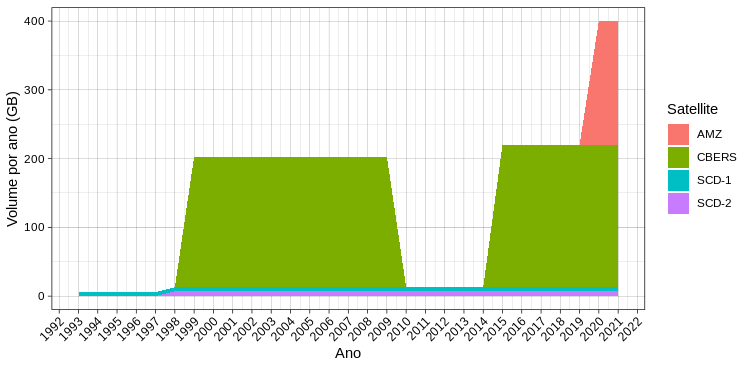
\includegraphics{Figuras/DataGenSatYear.png}}
	\end{center}
	\vspace{2mm}
	\legenda{Volume estimado de geração de dados por cada ano de operação de cada satélite.}
	\FONTE{Produção do autor.}
\end{figure}

Dessa estimativa, podemos obter o total de dados de telemetria disponíveis para a análise no CCS considerando uma taxa constante dos satélites, apresentados na figura~\ref{fig:totaldatagen}.
É importante ressaltar que a grande maioria desses dados não está disponível para consulta pelo usuário, visto que somente os dados de alguns poucos anos da operação estão disponíveis para os operadores e engenheiros, necessitando de trabalho significativo para analisar dados do passado.

\begin{figure}[!hb]
	\caption{Estimativa do volume de dados histórico de telemetria de todos os satélites}\label{fig:totaldatagen}
	\vspace{4mm}
	\begin{center}
		\resizebox{13cm}{!}{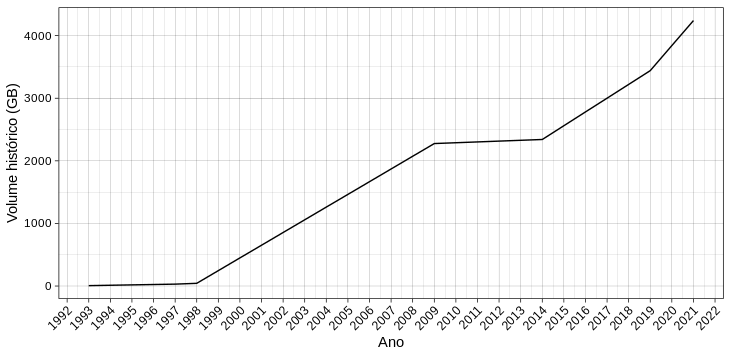
\includegraphics{Figuras/VolumeToYear.png}}
	\end{center}
	\vspace{2mm}
	\legenda{Volume total estimado de dados de telemetria gerados por todos os satélites.}
	\FONTE{Produção do autor.}
\end{figure}

Esses dados devem ser propriamente tratados para que não virem ``\textit{dark data}'', termo que denota quaisquer tipo de dados que não são de fácil acesso para os seus usuários em potencial~\cite{heidornSheddingLightDark2008}.

Esses dados entram na definição de \textit{Big Data}, pois possuem um grande volume, são gerados continuamente, possuem formatos diversos, sua análise é de alto valor e existe uma incerteza quanto a qualidade dos dados devido a problemas de comunicação e degradação dos instrumentos.
Essas características são denotadas pelos cinco Vs do \textit{Big Data}: Volume, Variedade, Velocidade, Valor e Veracidade~\cite{kacfahemaniUnderstandableBigData2015}.

Considerando que todos os dados já estivessem no banco de dados, propriamente formatados e prontos para a análise, ainda teríamos grandes problemas: com um banco de dados na ordem dos \textit{terabytes}, consultas multidimensionais ou que precisem de dados de vários anos poderiam demorar dias, ou mais, para serem executadas.

}

Deste modo, é necessário criar uma estrutura que permita a análise e consulta desses dados de uma forma estruturada e que tenha desempenho satisfatório.
As tecnologias de \textit{Data Warehouse} (DW) e \textit{Online Analytical Processing} (OLAP) tem demonstrado capacidade e experiência para atingir esses objetivos~\cite{bimonteOpenIssuesBig2016}, inclusive na área espacial~\cite{yvernesCopernicusGroundSegment2018}.
Essas tecnologias executam a generalização de dados agregando enormes quantidade de dados em vários níveis de abstração, assim tornam elementos essenciais de apoio à decisão e atraem a atenção tanto da indústria como das comunidades de pesquisa.
Sistemas OLAP, que são tipicamente dominados por consultas complexas que envolvem operadores \textit{group-by} e operadores de agregações, são as principais características entre essas ferramentas.

Sistemas OLAP são baseados em um modelo multidimensional chamado de cubo de dados, que é uma generalização do operador \textit{group-by} sobre todas as combinações possíveis das dimensões, com variados níveis de granularidade~\cite{grayDataCubeRelational1996}.
Cada combinação é chamada de um subcubo, que correspondem a um conjunto de células descritas como tuplas sobre as dimensões do subcubo.
Além das dimensões, cada tupla contém um fato, também chamado de medida, que representa o que será medido no processo de análise.

Cada dimensão pode estar organizada em uma hierarquia para facilitar a análise.
Por exemplo, uma dimensão tempo pode ser dividida em ``dia < mês < ano'', com ano sendo o nível mais genérico.
Essa prática visa facilitar a interpretação dos dados pelos usuários.
Medidas são atributos atributos associados a uma combinação de dimensões, sendo geradas de forma estatística.

Tecnologias OLAP são caracterizadas pela habilidade em responder consultas de apoio a decisão de forma eficiente.
Para atingir isso, o cubo de dados deve ser materializado antes da execução da consulta.
Isso significa que as combinações de dimensões são computadas previamente, assim gerando o cubo de dados completo.
Porém, essa abordagem possui um custo computacional exponencial em relação ao número de dimensões, assim a materialização completa do cubo envolve um grande número de células e um tempo substancial para a sua execução.

Dados de satélite são caracterizados pela sua alta dimensionalidade, onde um satélite pode precisar rastrear milhares de telemetrias.
Por exemplo, supondo um satélite com $n = 100$ telemetrias, e cada telemetria representando uma dimensão, teremos $2^{100}$ possíveis subcubos para a implementação de um cubo de dados.
Supondo uma cardinalidade, o número de valores diferentes em cada telemetria, como sendo de $100$, teremos $101^{100} \approx 10^{200}$ células para cada dimensão.
{\color{cerulean}
Devido ao controle ativo pelos operadores de satélite, os dados são concentrados em alguns valores que se repetem frequentemente, sendo que isso é chamado de \textit{skew}.
}

Dessa forma, conseguir calcular e manter um cubo de dados é um problema exponencial, e reduzir o seu consumo de memória e tempo de computação é de fundamental importância para desenvolver um sistema OLAP.
Para a área espacial essa necessidade é maior: a maior parte dos algoritmos de computação do cubo tem problemas em lidar com mais do que 15 dimensões~\cite{silva:2015:abordagensParaCubo}.

\section{Objetivos}\label{ch:intro:obj}

{\color{cerulean}

Assim, este trabalho tem como objetivo estabelecer um método para processamento de cubos de dados para a área espacial, para que o processamento de consultas OLAP sejam executadas de forma eficiente considerando-se a alta dimensionalidade, elevado número de tuplas, alto \textit{skew} e alta cardinalidade dos dados.

Assim é necessário identificar quais são as consultas de interesse dos operadores de satélite e quais são as análises que devem ser feitas pelos mesmos.
Disso será criada uma representação dimensional dos dados de telemetria em uma estrutura do cubo de dados, e  algoritmos de construção do cubo devem ser avaliados para identificar qual é o mais apropriado para responder as consultas.

Como resultados esperados deste trabalho teremos a avaliação dos algoritmos de construção do cubo nos dados altamente dimensionais, teremos as consultas identificadas e a adequabilidade do uso de cubo de dados como uma solução para operadores de satélites.

}

\section{Organização da proposta}\label{ch:intro:org}

Os capítulos restantes desta proposta estão organizados da seguinte maneira:

\begin{itemize}
	\item{Capítulo 2}: Este capítulo apresenta os conceitos e fundamentos teóricos desta proposta, como os conceitos relevantes de operação de satélites, \textit{Data Warehouse}, \textit{Big Data} e do Cubo de Dados.
	\item{Capítulo 3}: Neste capítulo os trabalhos correlatos de Cubo de Dados são apresentados, bem como as arquiteturas que outros operadores de satélite estão implementando.
	\item{Capítulo 4}: Neste capítulo a proposta é apresentada e seus conceitos principais explicados.
	\item{Capítulo 5}: Esse capítulo apresenta os resultados alcançados até o momento.
	\item{Capítulo 6}: Com base nos resultados intermediários alcançados, esse capítulo apresentará as conclusões obtidas, bem como as direções de implementação para o resto do trabalho.
\end{itemize}


%%%%%%%%%%%%%%%%%%%%%%%%%%%%%%%%%%%%%%%%%%%%%%%%%%%%%%%%%%%%%%%%%%%%%%%%%%%%%%

\chapter{THEORETICAL BACKGROUND}\label{ch:fun}

This chapter presents the theoretical background necessary to understand the concepts in this thesis, starting with satellite operations, the definitions of Big Data, Data Warehouse, OLAP and Data Cubes.

\section{Satellite Operations}\label{ch:fun:operations}

A satellite is divided into two modules: the service module and the payload.
The service module is composed of everything necessary for the operation of the on-board equipment, such as the power supply system, the ground communication system, the on-board computer, etc.
The payload is composed of all the necessary equipment to fulfill the mission objectives, these being sensors, cameras, telescopes, etc~\cite{larsonSpaceMissionAnalysis1999}.

A satellite generates two different types of data: payload data and telemetry data.
Payload data is the data generated to fulfill the mission of the satellite, and it can be photos taken for remote sensing, photos taken by telescopes, communication data if this is the focus of the mission among others~\cite{larsonSpaceMissionAnalysis1999}.
The telemetry data are the monitoring data of the health status and good operation of the satellite systems. These data are collected by the satellite's on-board computer, and are sent to the ground stations via telecommunication systems.

The telemetry data usually consist of sensor measurements on the satellite equipment, information collected by the on-board computer (such as whether an instrument is turned on or not), and other data whose collection has been defined as relevant to the operation of the satellite.
Depending on the mission, other measurements can be classified as telemetry, e.g. satellite-facing cameras, radars for the detection of possible collisions, etc~\cite{kragCmSpaceDebris2017}.

This data must be analyzed by satellite operators, who are responsible for monitoring and operating the satellite, on the ground after reception at the control center.
This analysis aims to ensure that the satellite is performing the tasks as it should, and that its state of health allows the continuation of the mission.

\section{Big Data}\label{ch:fun:bigdata}

The concept of Big Data is still evolving, and in this work the 5 Vs definition will be used: Volume, Variety, Velocity, Value and Veracity~\cite{kacfahemaniUnderstandableBigData2015}.

\begin{itemize}[noitemsep]
  \item \textbf{Volume}: This term generally specifies an amount of data in which a traditional database management system is ineffective.
  It is important to note that this is not only about the storage of data, but also about its processing~\cite{boussoufBigDataBased2018}.
  Using a large volume of data usually implies in better models, which are then hoped to produce better analyses, justifying the collection of a large amount of data.
  \item \textbf{Variety}: The data has multiple sources, with different formats, without a standardized modeling scheme, such as data coming from computertexts, sensor data, multimedia data, etc.
  As a consequence, these data should be used as transparently as possible in the analysis.
  \item \textbf{Velocity}: data is made available very quickly, and should be analyzed as quickly as possible.
  This implies that the data might be stored and analyzed even in real time.
  \item \textbf{Value}: data must be stored to create some value for its users, be it economic, scientific, social, organizational, etc.
  \item \textbf{Veracity}: the data has no guarantees as to its quality, such as inconsistencies and lack of accuracy, but the analysis must be of high quality anyway.
\end{itemize}

These V's are related to the construction of a Data Warehouse, and can also be seen as requirements for the creation of one for a data set characterized by Big Data~\cite{zhangBigDataFramework2017}.
In particular, there is a certain relationship with the idea of ``NoSQL'' (``Not only SQL''), where not only relational database systems are used, but also other paradigms are used, such as document oriented, key and value, etc~\cite{bimonteOpenIssuesBig2016}.

\section{Data Warehouse}\label{ch:fun:dw}

A Data Warehouse (DW) is a subject oriented, integrated, time-varying or time partitioned, non-volatile data repository that assists the decision making process~\cite{inmonUsingDataWarehouse1994}.
This definition can be divided into:

\begin{itemize}[noitemsep]
  \item \textbf{Subject oriented}: the DW is used for the analysis of a specific area.
    For example, a DW for telemetry data might just be useful for the operators, but not specific enough for engineering.
  \item \textbf{Integrated}: the DW must integrate data from multiple sources in a structured way.
    For example, even if there are two different representations for the same product, the DW should have only one representation.
    This requires the use of data cleaning and integration techniques in order to ensure data consistency.
  \item \textbf{Time-varying or time partitioned}: the DW must explicitly or implicitly contain the time perspective.
    This means that DW has historical data and they can be consulted during the analysis.
    For example, one might want to know data from days, months or years ago.
  \item \textbf{Non-volatile}: once inside DW, the data is not removed or updated, being a requirement for consulting historical data.
\end{itemize}

These features differentiate the Data Warehouse from other repository systems such as database systems, transaction processing systems and file systems~\cite{hanDataMiningConcepts2011}.

A DW is generally represented by a dimensional model that allows efficiency in data organization and management information retrieval~\cite{kimballDataWarehouseToolkit2013}.
Furthermore, this model has a few definitions: facts, dimensions and measures.
A fact corresponds to the business subject to be analyzed, each dimension is a visualization perspective of the business subject and measures are numerical values that quantify the business subject.
One of the dimensions is always temporal to allow the analysis of the subject over time.

\section{OLAP}\label{ch:fun:olap}

\textit{On-line Analytical Processing} (OLAP) is a term that refers to a set of tools that are used to summarize, consolidate, visualize, apply formulations and synthesize data according to multiple dimensions~\cite{coddProvidingOlapUseranalysts1998}.

An OLAP system allows the response of multi-dimensional queries using data stored in the Data Warehouse~\cite{kimballDataWarehouseToolkit2013}, and the main features are~\cite{bimonteOpenIssuesBig2016}:

\begin{itemize}[noitemsep]
  \item \textbf{Online queries}: must be made \textit{Online}, that is, in time for the user.
  \item \textbf{Multidimensional queries}: They are defined using the dimensions and measures provided by the Data Warehouse, which expect high quality data.
  \item \textbf{Simple representation}: Query results must be represented using tables and graphs, because end users are usually decision makers who need visualizations that are relevant to the subject.
  \item \textbf{Exploratory}: queries are used in an exploratory way, since users generally do not know in advance all the data available for queries.
\end{itemize}

Each OLAP tool must manipulate a new Abstract Data Type (ADT), called a data cube, using specific strategies due to the way the data is stored, being classified in~\cite{moreiraFullPartialData2012}:

\begin{itemize}[noitemsep]
  \item \textbf{Relational OLAP (ROLAP)}: use relational Database Management Systems (Data base Management System - DBMS) for the management and storage of data cubes.
    ROLAP tools include optimizations for each DBMS, implementation of navigation logic in aggregations, services and additional tools;
  \item \textbf{Multidimensional OLAP (MOLAP)}: implement multidimensional data structures to store data cubes in main memory or in external memory.
    No relational repositories are used to store multidimensional data and the navigation logic is already integrated into the proposed structure;
  \item \textbf{Hybrid OLAP (HOLAP)}: combine ROLAP and MOLAP techniques, where detailed data is stored in a relational database (ROLAP), and aggregations are stored in multidimensional data structures (MOLAP).
\end{itemize}

It is important to highlight the difference between OLAP and Online Transaction Processing (OLPT), since common database systems use only OLTP, which has the purpose of performing valid transactions and processing queries.
This covers the vast majority of day-to-day operations, such as stock control, banking operations, etc., serving various users of an organization.
OLAP is used by decision makers and data analysts and is geared towards higher level decisions in the organization~\cite{hanDataMiningConcepts2011}.

\section{Data Cube}\label{ch:fun:cube}

The data cube was originally created as a relational operator that generates all the possible combinations of its attributes according to a measure~\cite{grayDataCubeRelational1996}.

The structure of the data cube allows the data to be modeled and visualized in multiple dimensions, and it is characterized by dimensions and measures.
A measurement is an attribute whose values are calculated by the relationship between the dimensions, which is calculated using aggregation functions such as sum, count, average, mode, median, etc.
A dimension is made by the entities that compose the data, determining the context of the subject in question.
A dimension can also be divided into members, which can have a hierarchy, such as a time dimension divided in day, month and year~\cite{hanDataMiningConcepts2011}.

The organization of a data cube allows the user the flexibility to visualize the data from different perspectives, since the cube operator generates combinations through the concept of the value \textit{ALL}, where this concept represents the aggregation of all possible combinations of a set of attribute values.
Operations in data cubes exist in order to materialize these different views, allowing search and interactive analysis of stored data~\cite{hanDataMiningConcepts2011}.

A data cube is composed of cells and each cell has values for each dimension, including \textit{ALL}, and values for the measurements.
\autoref{fig:cubeexample} shows an example of a data cube.
The value of a measure is computed for a given cell using lower aggregation levels to generate the values of the higher aggregation levels in the \textit{Top-down} strategy, with the inverse order used in \textit{Bottom-up}.

\begin{figure}[!htb]
  \caption{Data Cube example}\label{fig:cubeexample}
  \vspace{2mm}
  \begin{center}
    \resizebox{9cm}{!}{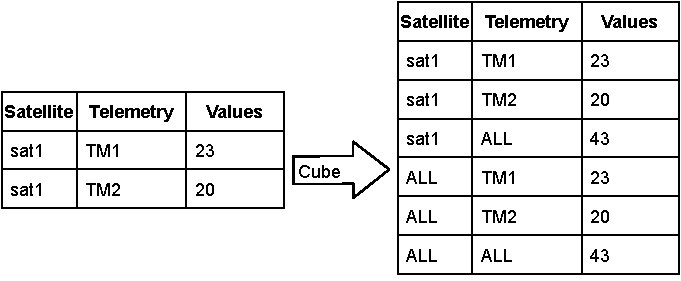
\includegraphics{Figuras/CubeExample.pdf}}
  \end{center}
  \vspace{1mm}
  \legenda{}
  \FONTE{Author}
\end{figure}

\subsection{Data Cube Cells}\label{ch:fun:cube:cells}

A data cube is composed of several subcubes, which are all possible levels of aggregation in the specified dimensions.
Subcubes are composed of base cells and aggregated cells, and an aggregated cell is a cell that uses the special value \textit{ALL} (``$*$'') to demonstrate that it is adding values in one or more dimensions.
A base cell does not use the \textit{ALL} notation, being composed of the lowest level of aggregation~\cite{limaSEQUENTIALPARALLELAPPROACHES2009}.
\autoref{fig:hasse} shows all levels of aggregation of a cube composed of dimensions A, B and C, from the most generic (\textit{apex}) to the most specific (base).

\begin{figure}[!htb]
  \caption{All subcubes for a three dimensional cube}\label{fig:hasse}
  \vspace{2mm}
  \begin{center}
    \resizebox{5cm}{!}{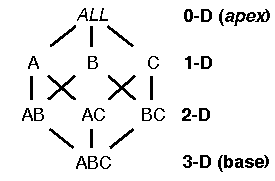
\includegraphics{Figuras/Hasse.pdf}}
  \end{center}
  \vspace{1mm}
  \legenda{A Hasse Diagram of a data cube with three dimensions A, B and C.}
  \FONTE{Author}
\end{figure}

Formally, assuming a $n$-dimensional data cube, a cell $a$ of any subcube is defined by $a = (a_1, a_2, a_3, \ldots, a_n, measures)$.
The cell is $m$-dimensional (from a subcube with $m$ dimensions), if exactly $m$, with $(m \leq n)$, values between $(a_1, a_2, a_3, \ldots, a_n)$ are not ``$*$''.
If $m = n$, then $a$ is a base cell, otherwise $(m < n)$, it is an aggregate cell.

A descending-ancestral relationship can exist between cells.
In a $n$-dimensional data cube, a cell $a = (a_1, a_2, a_3, \ldots, a_n, measures_a)$ with level $i$ is an ancestor of a cell $b = (b_1, b_2, b_3, \ldots, b_n, measures_b)$ of level $j$, and $b$ is a descendant of $a$, if and only if $i < j$ and $1 \leq m \leq n$, where $a_m = b_m$ whenever $a_m \neq *$.
In particular, a $a$ cell is called the parent of a $b$ cell, and $b$ the child of $a$, if and only if $j = i+1$ and $b$ is a descendant of $a$~\cite{hanDataMiningConcepts2011}.

\subsection{Dimensional Modelling}\label{ch:fun:cube:dimm}

There are three main schemes for the dimensional modeling of a data cube: Star Schema, Snowflake Schema and Fact Constellation.
The star schema is the most used, as it contains a central table called the fact table, where most of the data is located, with a smaller set of tables, called dimension tables, for the other dimensions.
\autoref{fig:starschema} shows an example of a star scheme.

\begin{figure}[!htb]
  \caption{Star schema}\label{fig:starschema}
  \vspace{6mm}
  \begin{center}
    \resizebox{4cm}{!}{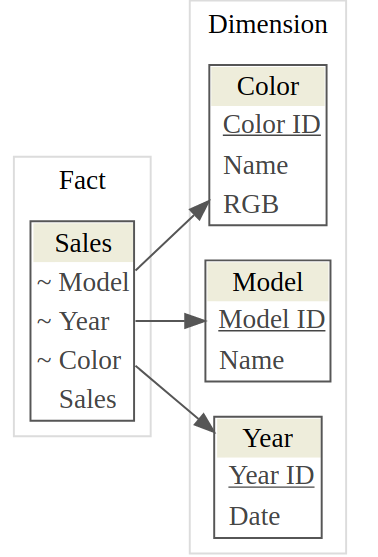
\includegraphics{Figuras/starSchema.png}}
  \end{center}
  \vspace{1mm}
  \legenda{}
  \FONTE{Author}
\end{figure}

The snowflake scheme is a variation of the star scheme, where some dimensions are normalized, dividing the data of the dimension tables into other tables.
This has the advantages of eliminating redundancies in the dimension tables, but it creates problems during the execution of queries since it is necessary to perform join operations with the new tables.
\autoref{fig:snowflakeschema} shows an example of a snowflake scheme.

\begin{figure}[!htb]
  \caption{Snowflake schema}\label{fig:snowflakeschema}
  \vspace{2mm}
  \begin{center}
    \resizebox{6cm}{!}{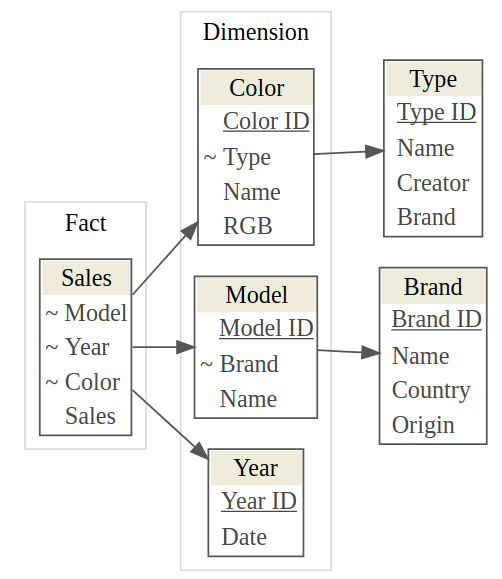
\includegraphics{Figuras/snowflakeSchema.png}}
  \end{center}
  \vspace{1mm}
  \legenda{}
  \FONTE{Author}
\end{figure}

The Fact Constellation uses multiple fact tables, like multiple star schemas but sharing dimension tables, leading to its name as a group of stars.
\autoref{fig:factconstschema} shows an example of a fact constellation scheme.

\begin{figure}[!htb]
  \caption{Fact Constellation scheme}\label{fig:factconstschema}
  \vspace{6mm}
  \begin{center}
    \resizebox{6cm}{!}{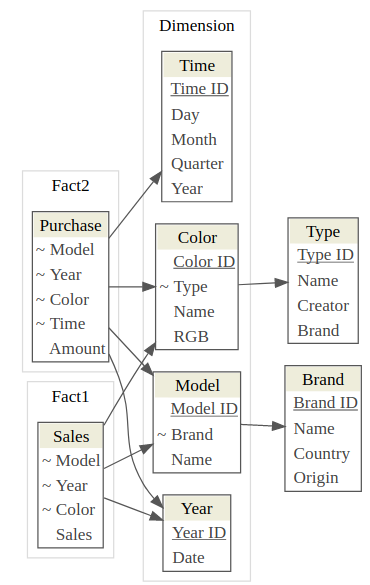
\includegraphics{Figuras/factConstellationSchema.png}}
  \end{center}
  \vspace{2mm}
  \legenda{}
  \FONTE{Author}
\end{figure}

\subsection{Concept Hierarchies}\label{ch:fun:cube:concept}

A concept hierarchy is used to define a mapping sequence between a set of low-level concepts and a set of high-level, more general concepts.
It is a style of grouping and discretization, because it groups the values in order to reduce the cardinality of a dimension~\cite{hanDataMiningConcepts2011}.
They help make the analysis easier to understand, as the operations translate the low-level data into a representation that is easier for the end user, thus facilitating the execution of queries and their subsequent use.

\subsection{Measures}\label{ch:fun:cube:measures}

Each cell of a cube is defined as a pair $\langle (d_1, d_2, \ldots, d_n), measures \rangle$, where $(d_1, d_2, \ldots, d_n)$ represent the possible combinations of attribute values over dimensions.
A measure is calculated for a certain cell by aggregating the data corresponding to the combination of dimensions and values~\cite{hanDataMiningConcepts2011}.
Measurements can be classified into three types: distributive, algebraic and holistic.

A distributive measure is a measure whose calculation can be partitioned and then combined, and the result would be the same if the calculation was performed on the entire data set.
For example, the sum function is distributive: dividing the $N$ data into $n$ sets, and making the sum of each $n$ set, will have the same result as if it were done directly over $N$.

An algebraic measure is a measure that can be calculated with two or more distributive measures.
For example, a measure of average can be calculated by dividing the measure sum by the measure count, which are both distributive.

A measure is holistic if there is no algebraic measure with $M$ arguments that performs the computation.
This means that computing cannot be partitioned, with exact values obtained only if the measure is applied to all data.
Some examples are the measures of mode, standard deviation and median~\cite{hanDataMiningConcepts2011}.

\subsection{OLAP Operations}\label{ch:fun:cube:olapops}

To perform queries in the Data Warehouse, it is necessary to use some operations on the data cube to obtain the appropriate results.
These queries must also be able to go through the hierarchy of concepts of each dimension, as well as follow the dimensional model of the cube, in order to offer a user-friendly interface for interactive analysis~\cite{hanDataMiningConcepts2011}.
Some operations are exemplified in \autoref{fig:olap}, but they usually are:

\begin{itemize}[noitemsep]
  \item \textit{Roll-up}: performs aggregation in the data cube, either by navigating the concept hierarchy from a specific level concepts to a more generic one, or by reducing a dimension.
  \item \textit{Drill-down}: the inverse of the roll-up operation, navigates in the hierarchy of concepts from the most generic level to the most specific level, or adds dimensions to the current cube.
  \item \textit{Slice}: performs a selection in a cube dimension, resulting in a subcube focused on that dimension.
  \item \textit{Dice}: defines a subcube by making a selection (slice) in two or more dimensions.
  \item \textit{Pivot}: also called rotation, it allows changing the position of the dimensions in view, changing rows to columns and vice versa.
\end{itemize}

\begin{figure}[!htb]
  \caption{OLAP operations in a Data Cube}\label{fig:olap}
  \vspace{4mm}
  \begin{center}
    \resizebox{15cm}{!}{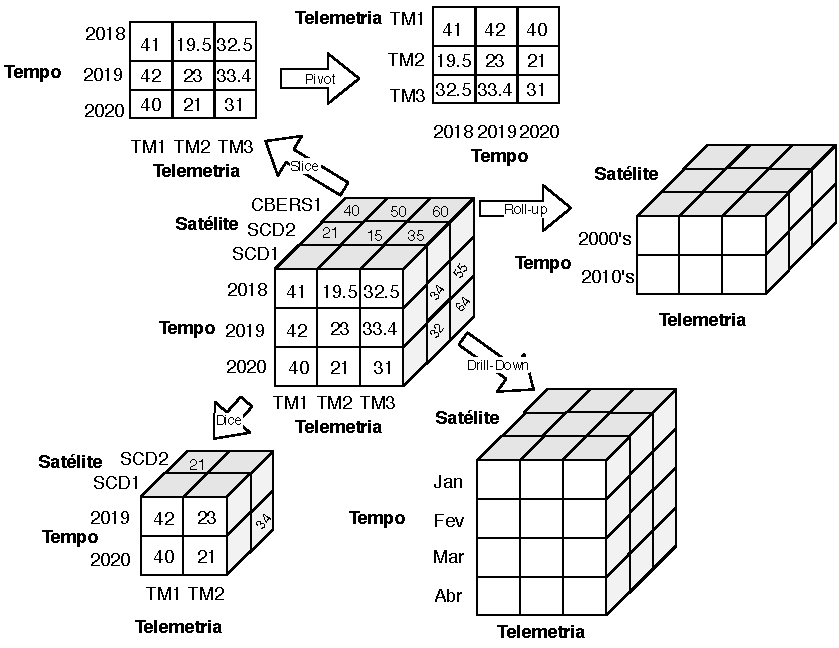
\includegraphics{Figuras/OLAP.pdf}}
  \end{center}
  \vspace{2mm}
  \legenda{Common OLAP operations on a three-dimensional data cube with Satellite, Time and Telemetry dimensions}
  \FONTE{Author}
\end{figure}

Depending on the OLAP system, it is possible to execute other operations, like drill-across between multiple fact tables, and drill-through where queries are executed directly on the low-level representation of the data~\cite{hanDataMiningConcepts2011}.

\subsection{Data Cube Computation}\label{ch:fun:cube:comp}

Data cube computation is an essential task, as pre-computing all or part of a data cube can significantly increase DW performance.
However, this task has exponential complexity in relation to the number of dimensions, being called materialization, with complete materialization requiring a large number of cells, and therefore a high consumption of memory and time~\cite{hanDataMiningConcepts2011}.

The original calculation of the data cube computation was proposed by~\citeonline{grayDataCubeRelational1996}, being: given an input relation $R$ with tuples of size $n$, the number of subcubes that can be generated is $2^n$, where $n$ is the number of dimensions of the cube.
For example, assuming a cube with three dimensions \textit{Satellite, Telemetry, Value}, we have $2^3 = 8$ possible subcubes: $\{(satellite, telemetry, value), (satellite, value), (satellite, telemetry),$ $(telemetry, value), (telemetry), (value), (satellite), \emptyset \}$, with $\emptyset$ denoting the empty grouping (base cell, dimensions are not grouped).
% Weird latex thing here...

However, in practice, dimensions can have associated concept hierarchies, as for the time dimension: ``day<month<quarter<semester<year'.
For a cube with $n$ dimensions with multiple concept hierarchies, the total number of subcubes is shown in \autoref{eq:conceptcuboids}.

\begin{equation}
  subcubes = \prod_{i=1}^n (L_i + 1)
\label{eq:conceptcuboids}
\end{equation}

Where $L_i$ is the number of concept levels of the $i$ dimension.
It is necessary to add one to the equation~\ref{eq:conceptcuboids} to denote the virtual level \textit{ALL}.
The size of each subcube also depends on the cardinality of each dimension, that is, the number of distinct values.
While the number of dimensions, concept hierarchies, and cardinality of the cube increases, they also increase the space requirements exponentially, being known as the \textbf{Curse of Dimensionality} in computing.

To be able to answer the queries properly, it is necessary to choose a method for subcube computing: non-materialisation, complete materialisation and partial materialisation.

In non-materialisation, the aggregated subcubes are not pre-computed, so the aggregations are computed in query time, which can be extremely slow, but has the lowest memory consumption.

Complete materialization computes all possible aggregations of the cube, generating a complete data cube.
This method generates the best response times, because the aggregations have already been computed, but it requires a large amount of memory.

Partial materialization only computes a selected subset of subcubes, and there are several different techniques for selecting the subcubes to be computed.
One of them is to compute all the subcubes that contain only cells that satisfy a given criterion, specified by the user.
These cubes are called iceberg~\cite{beyerBottomupComputationSparse1999}.

Another technique is to compute small cubes, usually between 3 and 5 dimensions, to form complete cubes.
To answer queries with more dimensions, the combinations between the small subcubes are aggregated.
This technique is called shell fragment, and the cube is called cube shell~\cite{liHighdimensionalOLAPMinimal2004}.

A data cube where cells with identical measurements are encapsulated in a single abstraction, called a closed cell is called a closed cube~\cite{dongxinCCubingEfficientComputation2006}, or quotient cube~\cite{lakshmananQuotientCubeHow2002}.

The choice of partial materialization depends on the required balance between response time and storage space.
However, full cube computation remains relevant, and advances in partial cube computation are generally adopted in full cube computation.
There is also the problem of updating the cube, as each update can cause a partial or complete recomputation of the cube to maintain the correct measurements.

From a base cube, the data cube computation can use the Top-down or Bottom-up strategy for the generation of the remaining subcubes~\cite{hanDataMiningConcepts2011}.

\autoref{fig:topdown} shows the generation of a four-dimensional data cube by the Top-down strategy.
ABCD being a base cube, the three dimension subcubes are: ABC, ABD, ACD and BCD; which can use the results of the base cube to be computed.

\begin{figure}[!hbt]
  \caption{Computing the data cube with the Top-Down strategy}\label{fig:topdown}
  \vspace{4mm}
  \begin{center}
    \resizebox{7cm}{!}{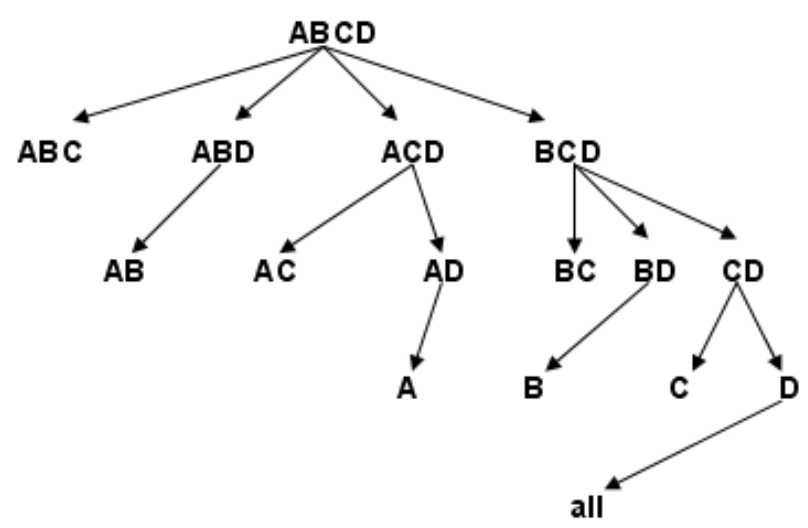
\includegraphics{Figuras/topdown.png}}
  \end{center}
  \vspace{2mm}
  \legenda{}
  \FONTE{~\cite{silva:2015:abordagensParaCubo}.}
\end{figure}

Os resultados da computação do subcubo ACD podem ser utilizados para computar AD, que consequentemente podem ser utilizados para computar A.
Essa computação compartilhada permite que a estratégia \textit{Top-down} compute agregações em múltiplas dimensões.
Os valores agregados intermediários podem ser reutilizados para a computação de subcubos descendentes sucessivos.

A Figura~\ref{fig:bottomup} mostra a geração de um cubo de dados de 4 dimensões por meio da estratégia \textit{Bottom-up}.
Subcubos de poucas dimensões tornam-se pais de subcubos com mais dimensões.
Infelizmente, a computação compartilhada, utilizada na estratégia \textit{Top-down}, não pode ser aplicada quando utilizada a estratégia \textit{Bottom-up}, então cada subcubo descendente necessita ser computado do início.

The results of the ACD subcube computation can be used to compute AD, which consequently can be used to compute A.
This shared computing allows the Top-down strategy to compute aggregations in multiple dimensions.
The intermediate aggregated values can be reused for the computation of successive descending subcubes.

\autoref{fig:bottomup} shows the generation of a 4-dimensional data cube through the Bottom-up strategy.
Low dimensional subcubes become parents of more dimensioned subcubes.
Unfortunately, the shared computing used in the Top-down strategy cannot be applied when using the Bottom-up strategy, so each descending subcube needs to be computed from the beginning.

\begin{figure}[!htb]
  \caption{Computing the data cube with the Bottom-Up strategy}\label{fig:bottomup}
  \vspace{4mm}
  \begin{center}
    \resizebox{8cm}{!}{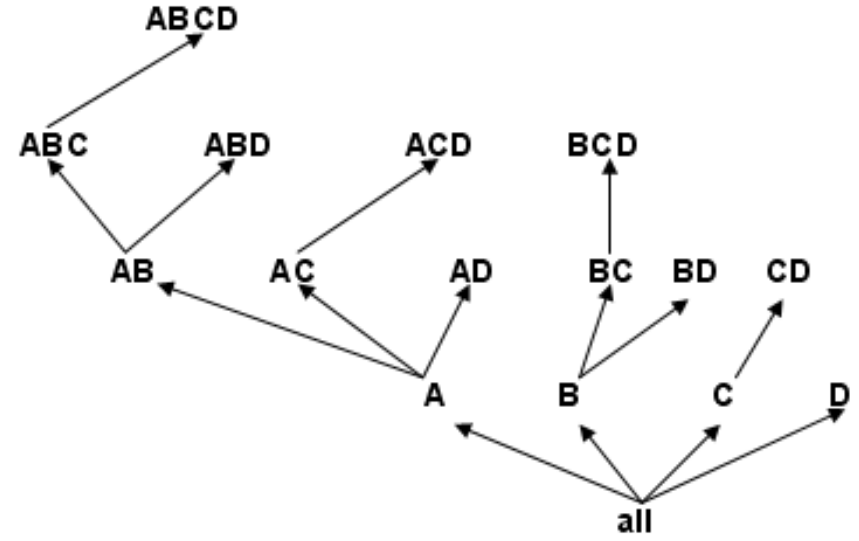
\includegraphics{Figuras/bottomup.png}}
  \end{center}
  \vspace{2mm}
  \legenda{}
  \FONTE{~\cite{silva:2015:abordagensParaCubo}.}
\end{figure}


%%%%%%%%%%%%%%%%%%%%%%%%%%%%%%%%%%%%%%%%%%%%%%%%%%%%%%%%%%%%%%%%%%%%%%%%%%%%%%%

\chapter{TRABALHOS CORRELATOS}\label{ch:corr}

Nessa seção, vamos apresentar os trabalhos correlatos a essa proposta.
Eles podem ser divididos em duas seções: as soluções de \textit{Big Data} de outros operadores, e os algoritmos de construção do cubo de dados com alta dimensionalidade.

\section{Dados da operação}\label{ch:prop:data}

A tabela~\ref{table:bigdatasattypes} mostra os tipos de dados relevantes para a operação, a sua origem e o seu formato esperado.
Essa tabela considera apenas dados considerados como telemetria do próprio satélite, ou dados advindos de terceiros.

\begin{table}[!ht]
	\begin{center}
		\caption{Dados de Operação}\label{table:bigdatasattypes}
		\begin{tabular}{|c|C{5cm}|c|}
			\hline
			\bfseries Tipo de Dado         & \bfseries Origem           & \bfseries Formato      \\
			\hline
			Sensores de bordo              & Equipamentos no satélite   & Tabelas, CSV           \\
			\hline
			Registros do Computador        & Computador de Bordo        & Texto (\textit{Logs})  \\
			\hline
			Multimídia                     & Câmeras                    & MP4, JPG, RAW          \\
			\hline
			Parâmetros orbitais            & Operação, Rastreio         & TLE, texto, tabelas    \\
			\hline
			Documentação associada         & Operadores, engenharia     & Texto (Word, Excel)    \\
			\hline
			Clima Espacial                 & Sensores no solo ou espaço & Texto, tabelas, avisos \\
			\hline
			\textit{Situational Awareness} & Radares, US-STRACOM, etc   & Texto, tabelas, avisos \\
			\hline
		\end{tabular}
	\end{center}
	\FONTE{Adaptado de~\cite{zhangBigDataFramework2017}}
\end{table}

Para este trabalho, apenas os dados vindos de sensores de bordo serão considerados.
Os outros dados nesta tabela poderiam ser considerados para uma \textit{Data Warehouse} mais completa, porém estão fora do escopo desta proposta.

\subsection{Fluxo dos Dados}\label{ch:prop:dataflow}

Baseado nos trabalhos correlatos e nos dados levantados, a figura~\ref{fig:bigdataflow} demonstra o fluxo de dados esperado de uma arquitetura de \textit{Big Data} para a operação de satélites.

\begin{figure}[ht]
	\caption{\color{red} Fluxo de dados em uma arquitetura de \textit{Big Data}}\label{fig:bigdataflow}
	\vspace{6mm}
	\begin{center}
		\resizebox{15cm}{!}{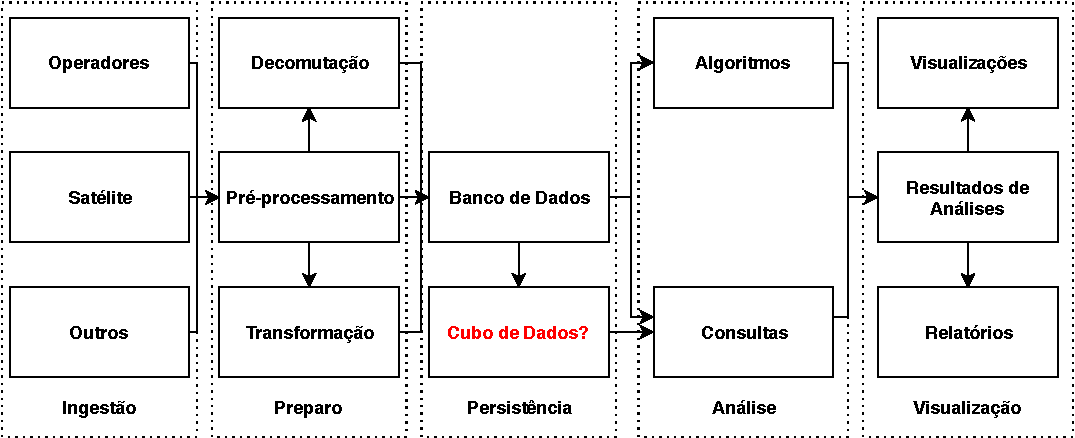
\includegraphics{Figuras/BigDataFlow.pdf}}
	\end{center}
	\vspace{2mm}
	\legenda{}
	\FONTE{Adaptado de~\cite{zhangBigDataFramework2017}}.
\end{figure}

Este fluxo está separado em cinco etapas que vão desde a origem dos dados até o seu resultado de análise, e este trabalho visa apenas mapear qual seria esse fluxo baseado nos trabalhos correlatos.
Cada uma das etapas está detalhada a seguir:

\begin{itemize}
	\item \textbf{Ingestão}: onde os dados serão coletados na sua fonte (satélites, sensores no solo, outras fontes, etc).
	      Essa etapa se importa em \textbf{onde} estão os dados e \textbf{como} coletá-los, bem como \textbf{quais} são os dados importantes de serem coletados.
	      A ``fonte'' aqui pode ser um serviço de terceiros, dentro da própria instituição ou disponível de outra forma.
	\item \textbf{Preparo}: os dados relevantes são selecionados, e transformações são realizadas para inserir os mesmos na base de dados.
	      Essa etapa se importa no formato específico dos dados, realizando operações de limpeza, verificação da qualidade e da relevância para a análise, entre outras.
	      O seu objetivo é garantir que os dados tem qualidade, relevância, e estão no formato adequado para a base de dados.
	\item \textbf{Persistência}: após o devido processamento, os dados de alta qualidade são guardados em uma base de dados, de onde ficarão disponíveis para a análise.
	      Nessa etapa um banco de dados é utilizado, se importando apenas em como esses dados estão guardados e como eles serão disponibilizados para as consultas e execução de algoritmos.
	\item \textbf{Análise}: nesta etapa são executadas as consultas e os algoritmos de interesse para a análise.
	      Podem ser desde consultas simples (``qual era o valor da telemetria X durante a passagem Y?''), a execução de algoritmos complexos (``preveja os valores da telemetria X para a próxima passagem'').
	\item \textbf{Visualização}: os resultados das consultas e algoritmos são visualizados.
	      Podem conter desde gráficos simples, como um histograma de uma telemetria, a relatórios complexos de um subsistema/satélite, bem como resultados de algoritmos.
\end{itemize}

Os trabalhos de~\cite{zhangBigDataFramework2017},~\cite{mateikUsingBigData2017} e~\cite{boussoufBigDataBased2018} definem esse processo mais claramente dentre os trabalhos apresentados.

\section{Análise de Dados em Outros Operadores de Satélite}\label{ch:corr:ops}

A tabela~\ref{table:bigdataoperators} mostra uma revisão feita em artigos recentes sobre os operadores de satélite e quais tecnologias eles estão utilizando para atingir objetivos semelhantes, principalmente com o uso de \textit{Big Data}.

\begin{table}[htbp]
	\begin{center}
		\caption{Operadores de Satélite e Arquiteturas de Big Data}\label{table:bigdataoperators}
		\begin{tabular}{|C{8em}|C{6em}|c|C{10em}|}
			\hline
			\bfseries Referência                           & \bfseries Operador & \bfseries Ferramenta & \bfseries Tecnologias                                                                \\
			\hline
			\cite{adamskiDataAnalyticsLarge2016}           & L3 (EUA)           & InControl            & Hadoop, Spark, HBase, MongoDB, Cassandra, Amazon AWS                                 \\
			\hline
			\cite{boussoufBigDataBased2018}                & Airbus             & Dynaworks            & Hadoop, Spark, HDFS, HBase, PARQUET, HIVE                                            \\
			\hline
			\cite{schulsterCHARTingFutureOffline2018}      & EUMETSAT           & CHART                & MATLAB, MySQL, Oracle                                                                \\
			\hline
			\cite{zhangBigDataFramework2017}               & SISET (China)      & -                    & Hadoop, HDFS, PostgreSQL, MongoDB, Logstash, Kibana, ElasticSearch, Kafka, MapReduce \\
			\hline
			\cite{yvernesCopernicusGroundSegment2018}      & Telespazio France  & PDGS                 & OLAP (DataCube), Saiku, Pentaho, Jaspersoft OLAP                                     \\
			\hline
			\cite{dischnerCYGNSSMOCMeeting2016}            & SwRI + NOAA        & CYGNSS MOC           & SFTP, -                                                                              \\
			\hline
			\cite{edwardsDealingBigData2018}               & EUMETSAT           & MASIF                & FTP, RESTful service, JMS Messague Queue, PostgreSQL                                 \\
			\hline
			\cite{evansDataMiningDrastically2016}          & S.A.T.E + ESA/ESOC & -                    & Java, CSV                                                                            \\
			\hline
			\cite{fenManagementOperationCommunication2016} & CSMT (China)       & -                    & não menciona as tecnologias                                                          \\
			\hline
			\cite{trollopeAnalysisAutomatedTechniques2018} & EUMETSAT           & CHART                & algoritmos ad-hoc, estudo de caso                                                    \\
			\hline
			\cite{gillesFlyingLargeConstellations2016}     & L-3                & InControl            & Amazon EC2, LXC, Nagios                                                              \\
			%\hline
			%\cite{highsmithSpaceLaunchSystem2015} & Boeing + NASA & - & lançadores, não é o foco da arquitetura \\
			\hline
			\cite{hennionBigdataSatelliteYearly2018}       & Thales Alenia      & AGYR                 & Logstash, Kafka, InfluxDB, ElasticSearch, Kibana, Grafana                            \\
			\hline
			\cite{mateikUsingBigData2017}                  & Stinger, NASA      & -                    & Logstash, ElasticSearch, Kibana, HDF5, CSV, R, Python, AWS, Excel                    \\
			\hline
			\cite{fernandezTelemetryAnomalyDetection2017}  & NASA               & MARTE                & R, CSV, ad-hoc                                                                       \\
			\hline
		\end{tabular}
	\end{center}
	\FONTE{Produção dos autores.}
\end{table}

Os objetivos em comum desses trabalhos são facilitar as atividades dos operadores por meio de algoritmos de detecção de anomalias e de verificação dos limites nos valores das telemetrias.
Alguns dos operadores dessa lista estão responsáveis pela operação de constelações de satélites complexos, como constelações de sensoriamento remoto, que faz necessário um certo nível de automação ou a operação contínua teria um custo inviável.

Nesses trabalhos, o uso dessas tecnologias é apenas para os operadores de satélite, pois em nenhum desses trabalhos eles estão na mesma estrutura de ingestão dos dados da carga útil, mesmo utilizando as mesmas tecnologias, como demonstrado em~\cite{mateikUsingBigData2017} e~\cite{adamskiDataAnalyticsLarge2016}.

Alguns desses trabalhos não utilizam de estruturas completas que seguem um fluxo de dados, como é o caso de~\cite{fernandezTelemetryAnomalyDetection2017} e~\cite{trollopeAnalysisAutomatedTechniques2018} que utilizam de scripts feitos de forma \textit{ad-hoc}, não mostrando uma visão da arquitetura completa do fluxo de dados e apenas a ferramenta utilizada para análise pontual.

O trabalho de~\cite{yvernesCopernicusGroundSegment2018} utiliza de estratégias OLAP e do Cubo de Dados, tendo utilizado uma modelagem dimensional para a operação de uma constelação de satélites, porém esse trabalho menciona apenas em alto nível a modelagem utilizada, e menciona que o trabalho foi somente na parte da modelagem dimensional e integração dos dados utilizando ferramentas já existentes.

\subsection{Análise de Dados no INPE}\label{ch:corr:inpe}

O INPE já realiza análise de dados em outros setores, inclusive sobre as telemetrias de satélite.
Os operadores devem monitorar os valores das telemetrias e informar a engenharia caso algum problema que não pôde ser corrigido aparece~\cite{TominagaFerrAmbr:2017:CoSaTe}.
Um exemplo está no trabalho~\cite{Magalhaes:2012:EsAvTe}, feito sobre uma falha no satélite CBERS-2, onde o modelo proposto visa melhorar o conhecimento sobre avalanche térmica nas baterias para impedir que isso aconteça novamente em outros satélites.
A motivação principal dos trabalhos da tabela~\ref{table:bigdataoperators} era a detecção de anomalias, que teve alguns algoritmos estudados em~\cite{AzevedoAmbrViei::EsSoTe}.

Outros setores, utilizam a análise de dados vindos da carga útil do satélite ou de agentes externos ao INPE, como dados de sensoriamento remoto, cuja análise não é trivial e também estão classificados como \textit{Big Data}.
~\citeonline{monteiroFRAMEWORKTRAJECTORYDATA2017} utilizam de conceitos de Big Data para análise de trajetórias de objetos;~\citeonline{ramosDistributedSystemsPerformance2016} demonstram o uso de softwares como o Hadoop para a análise de dados do clima espacial, com uma arquitetura relacionada as arquiteturas revisadas na seção anterior; e~\citeonline{SimoesCamaQuei:2018:DaAnMa} mostra uma arquitetura que utiliza de Cubo de Dados para a análise de séries temporais no sensoriamento remoto.

{\color{red} \bfseries
Rodrigo: posso tirar esse parágrafo/seção toda se não achar relevante. Eu queria mostrar aqui que apesar dos dados da carga útil e da plataforma serem diferentes, eles tem características parecidas e podem compartilhar de soluções.
}

\section{Computação do Cubo de Dados}\label{ch:corr:cube}

A computação seletiva do cubo de dados possui muitos algoritmos diferentes implementados, porém eles possuem dificuldades no trato de dados com muitas dimensões e no uso limitado da memória~\cite{hanDataMiningConcepts2011}.
Vamos mencionar alguns dos algoritmos de desenvolvimento mais recente e que são mais relevantes para esta proposta.

O \textit{FragCubing}~\cite{liHighdimensionalOLAPMinimal2004} apresenta o conceito de \textit{cube shells}, onde cubóides com poucas dimensões (de 3 a 5 neste exemplo) são calculados utilizando de índices invertidos, que funcionam apenas utilizando memória principal.

Precursor para o computação distribuída do cubo,~\cite{dokaBrownDwarfFullydistributed2011} apresenta o \textit{Brown Dwarf}, um sistema \textit{Peer-to-Peer} que permite atualização das células, desenhado para diminuir a redundância em cubos distribuídos.

O \textit{PopUp-Cubing} é apresentado em~\cite{heinePopUpCubingAlgorithmEfficiently2017}, que utiliza de icebergs para lidar com dados em formato de \textit{stream}, obtendo resultados superiores ao FTL e \textit{Star-Cubing}.
Este trabalho é de interesse especial por utilizar de dados de \textit{stream}, que permitiriam resultados parecidos com tempo-real, que são mais parecidos com os dados disponíveis para a operação de satélites.
Porém, não iremos abordar esse problema neste trabalho.

Com foco em \textit{Big Data} e utilizando como base o esquema \textit{MapReduce},~\cite{wangScalableDataCube2013} apresenta o algoritmo \textit{HaCube} para computação do cubo em paralelo.
Este trabalho apresenta um balanço entre computação do cubo em paralelo por vários nós de \textit{MapReduce}, que permite algumas atualizações e computação incremental de medidas.
Devido a própria natureza distribuída, ele precisa de mecanismos de tolerância a falha, e também os testes foram executados com no máximo apenas 5 dimensões, porém com até 2,4 bilhões de tuplas.
Ainda na linha do \textit{MapReduce},~\cite{yangHolisticAlgebraicData2017} demonstra a computação de medidas holísticas apresentando o \textit{Multi-RegionCube}, porém realizando menos testes que o \textit{HaCube}.

Em~\cite{zhaoClosedFragShellsCubing2018} é apresentado o \textit{Closed Frag-Shells Cubing}, que utiliza de uma combinação da abordagem de cubos fechados com a abordagem \textit{Shell fragments}, obtendo resultados melhores que a aplicação de cada uma delas separadamente.
Essa abordagem utiliza de índices \textit{bitmap} e índices invertidos, sendo que lidam com dados altamente dimensionais e sem uma hierarquia de forma similar ao necessário neste trabalho.

\textit{qCube}~\cite{silvaQCubeEfficientIntegration2013} extende a abordagem \textit{Frag-Cubing} para permitir consultas sobre intervalos de valor, extendendo os operadores de consultas clássicas em cubo de dados além do operador de igualdade.

\textit{HFrag}~\cite{silvaHybridMemoryData2015} apresenta o uso de memória externa na computação dos índices invertidos, utilizando de um sistema híbrido de memória para armazenar as partições do cubo tanto na memória principal quanto na secundária, com os valores mais frequentes sendo armazenados na memória principal e os valores menos frequentes na memória secundária.

A abordagem \textit{Hybrid Inverted Cubing} (HIC)~\cite{silvaComputingBIGData2016} extende a abordagem \textit{HFrag} com o parâmetro de frequência acumulada crítica, obtendo resultados melhores do que este nas mesmas consultas.

{\color{red} Falta a crítica nessa seção.}


%%%%%%%%%%%%%%%%%%%%%%%%%%%%%%%%%%%%%%%%%%%%%%%%%%%%%%%%%%%%%%%%%%%%%%%%%%%%%%%

\chapter{Experiment}\label{ch:experiment}

- The data available, how the next chapters are related and the brief description of the data come here.

- Also describe how the experiments will be performed and what will be measured. Basically the section of the results from the fragpaper.

The Frag-Cubing algorithm used the Illimine project implementation \cite{illimineSoftwareDataRepository} that was coded in C++ and compiled on a Linux Kernel 5.0.0-29 machine, with gcc 7.4.0.
Some adaptations were made to the original code to allow for better output formatting, however these were minimal format changes and didn't impact on the performance or changed how the algorithm works.
All of the experiments were executed on an Intel(R) Core(TM) i7-8550U CPU @ 1.80 GHz, with 16 GB of DDR4 @ 2400 MHz system memory and on an Adata XPG SX8200 Pro Solid State Drive using PCIe Gen 3x4 interface.

The experiments were designed to measure:

\begin{itemize}
\item Base cube main memory;
\item Runtime to build the base cube representation;
\item Query response time;
\item Query memory increase, which measures how much memory was needed to answer the query beyond what was used by the base cube.
\end{itemize}

As a notational convention, we use \(\mathcal{D}\) to denote the number of dimensions, \(\mathcal{C}\) the cardinality of each dimension, \(\mathcal{T}\) the number of tuples in the database, \(\mathcal{F}\) the size of the shell fragment, \(\mathcal{I}\) the number of instantiated dimensions, \(\mathcal{Q}\) the number of inquired dimensions, and \(\mathcal{S}\) the skew or zipf of the data.
Minimum support level is 1, as well as \(\mathcal{F} = 1\) for all experiments.
Due to random sampling of the data, it is assumed that the skew is \(\mathcal{S} = 0\) for all dimensions.

Each test was executed 5 times, with the average value of the five runs being taken.
Additionally, before each test a baseline with no performed queries was executed, just computing the time to cube: how long, and using how much memory, it takes for the algorithm to compute the initial cube.
This is meant to ease the comparison of the results.

The central idea of this experiment is to partition the input data with the dimensions with the expected dimensions used in a query, to see if that is a better or worse cube construction strategy.
To achieve that, the 4 year of data resulted in to 24 M (\(\ensuremath{2.4\times 10^{7}}\)) tuples over the satellite's 135 telemetries, saved in a relational database.
Those were separated into files for each query and each data size.
To better provide comparisons, each data was separated into datasets of equal interval: 2M, 4M, 6M, 8M and 10M tuples (\(\ensuremath{2\times 10^{6}}\), \(\ensuremath{4\times 10^{6}}\), \(\ensuremath{6\times 10^{6}}\), \(\ensuremath{8\times 10^{6}}\) and \(\ensuremath{10^{7}}\)).

In a first test run it was found that the different data distributions at those levels were interfering with the experiment, and so, to evaluate only the general distribution of the data and how it was organized, each tuple of each dataset was sampled at random for the full \(\ensuremath{2.4\times 10^{7}}\) original data.
This leads to complete random data between each number of tuples, but no variance between the selected columns for each query, allowing them to be compared.

In the end, this resulted in $12,83$ GB of data converted to Frag-Cubing's format, counting the datasets with the full 135 telemetries and the datasets with the filtered telemetries, resulting in 30 different data files (5 for the high-dimensional case, and 5 for each query).

For this paper, the names in Table \ref{tab:cubenotation} will be used to refer to each of these cubes.
The cubes with 135 dimensions will be treated as ``C0'', with ``C1'' to ``C5'' being the cubes with dimensions filtered for the telemetries in ``Q1'' to ``Q5''.

\begin{table}[H]
\caption{Cube representation used in the experiment}\label{tab:cubenotation}
\centering
\begin{tabular}{cccp{1.5cm}}
\toprule
\bfseries ID &\bfseries Query &\bfseries Dimensions &\bfseries Total Size\\
    \midrule
    C0 & - & 135 & 11,29 GB \\
      C1 & Q1 & 6 & 0,44 GB \\
      C2 & Q2 & 3 & 0,34 GB \\
      C3 & Q3 & 2 & 0,22 GB \\
      C4 & Q4 & 2 & 0,20 GB \\
      C5 & Q5 & 3 & 0,34 GB \\
      \bottomrule
      \end{tabular}
      \end{table}

      The process to separate the data was performed as follows:

      \begin{enumerate}[leftmargin=*,labelsep=5.8mm]
      \item Select from telemetry database (PostgreSQL) the dimensions that are used in the query (ex. `SELECT TM001, TM002 FROM telemetries');
      \item Randomly select $n$ tuples from that selection, where $n$ is in \(\ensuremath{2\times 10^{6}}\), \(\ensuremath{4\times 10^{6}}\), \(\ensuremath{6\times 10^{6}}\), \(\ensuremath{8\times 10^{6}}\) and \(\ensuremath{10^{7}}\);
      \item Save the results to a file and convert it to Frag-Cubing's input format, naming it cube $i$ (eg. "C$i$"), where $i$ is one of the query identifiers;
      \item Load the file into Frag-Cubing and execute the relevant queries.
      \end{enumerate}



%%%%%%%%%%%%%%%%%%%%%%%%%%%%%%%%%%%%%%%%%%%%%%%%%%%%%%%%%%%%%%%%%%%%%%%%%%%%%%%

\chapter{QUERY PARTITION}\label{ch:querypart}

In this chapter, an algorithm for aggregating the satellite telemetries into relationship groups is presented, which is then used to selected useful queries for a satellite operator.
These queries are then compared with the Frag-Cubing algorithm: one set is called High-Dimensional, in which the queries are executed on the full data dimensionality; and the other is Low-Dimensional, in which the input data for the data cube algorithm is made of only the dimensions that the query will execute.
The aim of this work is then to see if the query response time and memory consumption can be improved by pre-filtering the data that will be searched with just the dimensions related to the query.

\section{Algorithm}\label{ch:querypart:heur}

The objective of this algorithm is to easily classify the rate of change between groups of telemetries, as from previous data science work conducted on the telemetry data, just by identifying whether a group of telemetries changing on a similar rate, it is possible to find a relationship between them.
The algorithm is separated into two parts: the groups generation and the strength calculation.

\hypertarget{aggregation-generator}{%
\subsection{Aggregation generator}\label{ch:querypart:heur:agg}}

The algorithm works by creating telemetry groups with all possible dimensional combinations, considering each telemetry as a dimension.
The combination of a given set of \textbf{n} elements taken \textbf{k} at a time is given by formula \ref{eq:cardinalitygeneral}.

\begin{equation} \label{eq:cardinalitygeneral}
C_k^n = \binom{n}{k}
\end{equation}

Since the number of telemetries is usually on the order of hundreds to thousands, it's best to limit the algorithm to combinations taken from 2 to 5 at a time.
This is equivalent of computing all subcubes with those dimensions.
That gives us the following number of combinations, with \textbf{kmax} being the biggest \emph{k} that we want, on formula \ref{eq:kmax}.

\begin{equation} \label{eq:kmax}
\sum_{2\leq{k}\leq{n}}^{kmax}\binom nk = 2^{n-2}
\end{equation}

Each of these combinations is generated from a vector of \emph{n} telemetry names that we're interested.
For each of the generated combinations, we then execute aggregation measures:

\begin{itemize}[noitemsep]
\item
  Group the available telemetry readings by the combination groups
  \begin{itemize}
  \item
    for the combination ``TM001'', ``TM002'', group the table by ``TM001'' and ``TM002''
  \end{itemize}
\item
  Each aggregate is counted for frequency that the values appear, called \emph{count} henceforth

  \begin{itemize}
  \item
    TM001 = [``01''] \&\& TM002 = [``02''] -\textgreater{} count = 25
  \end{itemize}
\item
  For each of the telemetries used, compute the cardinality of the telemetry, called \(C_t\) for telemetry \emph{t}

  \begin{itemize}
  \item
    TM001 = [`01', `02',`03'], then it'll have cardinality 3
  \end{itemize}
\item
  Compute descriptive statistics over all the values of \emph{count}

  \begin{itemize}[noitemsep]
  \item Number of aggregates (length of the vector)
  \item Mean
  \item Median
  \item Standard deviation
  \end{itemize}
\end{itemize}

\hypertarget{relationship-strength-calculation}{%
\subsection{Relationship strength calculation}\label{ch:querypart:heur:rel}}

We can then use the descriptive statistics to calculate the strength of the relationship between the telemetries.
This involves the use of conditionals and some parameters from the algorithm.

The initial condition is that if the cardinality of any telemetry is 1, it means that it didn't change in the time period, hence any aggregate with \(C_t=1\) will be marked with \emph{NONE} on relationship.
If the number of groups is 1 it also means that no changes were observed in the period, so we can't infer any relationships from the data, and the relationship is marked \emph{NONE}.

If that condition passes, then we compute some values to help with classifying the other cases:

The biggest possible number of groups expected is the product of the sequence of cardinalities, called maxc is given by equation \ref{eq:maxc}.

\begin{equation} \label{eq:maxc}
    maxc = \prod_{t}C_t = C_1 * ... * C_t
\end{equation}

The biggest cardinality in the combination, to us the \emph{minimum} possible value for the number of groups, called \emph{minc} on equation \ref{eq:minc}.

\begin{equation} \label{eq:minc}
    minc = \max(C_1,...,C_t)
\end{equation}

The proportion of the number of groups by the maximum cardinality, called cratio on equation \ref{eq:cratio}.

\begin{equation} \label{eq:cratio}
    cratio = \frac{numgroups}{maxc}
\end{equation}

The absolute cardinality difference, as it is more representative of the discrepancy between bigger cardinalities, called \emph{abscdiff} on equation \ref{eq:abscdiff}.

\begin{equation} \label{eq:abscdiff}
    abscdiff = cratio - \frac{minc}{maxc}
\end{equation}

The coefficient of variation, from the standard deviation \(\sigma\) and the mean \(\mu\), called \emph{CV}, is used to check the variability of the number of groups inside an aggregate on equation \ref{eq:cv}.

\begin{equation} \label{eq:cv}
    CV = \frac{\sigma}{\mu}
\end{equation}

After all of those values, we are left with the choice of some parameters: the absolute cardinality ratio cutoff; the CV minimum and maximum cutoff and the CV minimum cutoff for the medium case.

Each of these parameters is necessary to characterize the distribution of each combination.
A high number of groups does not tell us much about its distribution: we need more statistics to know if the groups are evenly spread or if they are focused on few values.
Knowing that is essential to be able to distinguish the strength of the relationships.

So, the cardinality ratio cutoff is the first: it tells us how the cardinalities change in relation to each other.
The number \emph{cratio} will be closer to 1 if there's a relationship of 1 to 1 for each telemetry. This means that every time that one telemetry changes, the others changes too.

In contrast, a number closer to 0 means that the telemetries have very little variability, and that they're using the minimum expected cardinality.
This means that the number of groups is closer to \emph{minc}, and the variability is low.

The CV is then used to peer into the distribution of aggregates, by telling us if they're focused on few values or more spread evenly.
A value close to, or bigger than, one means that the data are very spread, and thus might have a strong relationship, as that means that they tend to change together.
A value closer to the CV minimum cutoff has data with low variability, which means that they're probably clustered together on few values.
If it's within the absolute cardinality variability cutoff, then this value also denotes a strong relationship.
If the value is within both cutoffs, then it's neither very clustered nor much variable, so we adopt a medium strength relationship.

From each of these paths, we have a single strength relationship, however the relative adoption of the relationship strength calculation is subjective, as the cutoff points need to be manually defined.
With this algorithm, some 2x2 and 3x3 relationships were generated by grid searching all possible relationships and then presented to a satellite operator for evaluation.

\section{Queries}\label{ch:querypart:queries}

With the satellite operator help, some sample queries that are frequent to the satellite operation procedures were filtered, not only related by their relationship but how useful the operator found them for their activities.
The related telemetries are summarized in ~\autoref{tab:telemetries}, with their identification, brief description and the calculated cardinality from the historic database.
In this table, the cardinality of each telemetry is defined as the number of unique values that the telemetry can take.

\begin{table}[H]
  \begin{center}
    \caption{Telemetries overview.}\label{tab:telemetries}
    \begin{tabular}{|c|p{6cm}|c|}
      \hline
      \textbf{ID} & \textbf{Description} & \textbf{Cardinality} \\
      \hline
      TM001 & Payload receiver voltage & 149 \\
      \hline
      TM002 & Payload RF output power & 175 \\
      \hline
      TM003 & Magnetometer 1, Y axis & 251 \\
      \hline
      TM004 & Magnetometer 1, -X axis & 251 \\
      \hline
      TM005 & Magnetometer 1, Z axis & 251 \\
      \hline
      TM006 & Magnetometer 2, Y axis & 251 \\
      \hline
      TM072 & Battery Temperature 1 & 251 \\
      \hline
      TM075 & Solar Panels Current & 251 \\
      \hline
      TM077 & Battery Charge Regulator 1 & 2 \\
      \hline
      TM078 & Battery Charge Regulator 2 & 2 \\
      \hline
      TM081 & Battery Temperature 2 & 251 \\
      \hline
      TM082 & Battery Discharge Regulator 1 & 2 \\
      \hline
      TM083 & Battery Discharge Regulator 2  & 2 \\
      \hline
      TM130 & Solar sensor temperature 1 & 233 \\
      \hline
      TM131 & Solar sensor temperature 2 & 233 \\
      \hline
    \end{tabular}
  \end{center}
\end{table}

\subsection{Q1}\label{q1}

Question: \textbf{are the batteries being charged or discharged?}

The related telemetries are: TM072 and TM081 are each of the satellite's battery thermistor readings, TM077 and TM078 are charge regulator telemetries for each of the batteries, and TM080 and TM081 are discharge regulator indicators for each battery.
The regulator telemetries simply indicate whether each battery is being charged or discharged as seen by the OBC, and take the form of ``ON'' and ``OFF'' values, while the thermistor telemetries indicate the thermal behavior of each battery.

This seems trivial at first glance: TMs 77, 78, 80 and 81 already display this information as each batteries' charge regulators, directly as collected by the OBC.
However, in the case of this satellite, the thermal behavior of the batteries is important to verify whether the batteries are actually being charged or not.
Furthermore, an overloading of one of the batteries might cause the relationship between the regulators to change and not show an accurate picture of what is happening, relating the query to anomaly discovery.

\subsection{Q2}\label{q2}

Question: \textbf{what is the current satellite orientation?}

The three telemetries are related to the magnetometer measurements, each (3, 4, 5) being of one axis (Y, X, Z) and with 300 mGauss precision.

This query has a simple objective of showcasing one of the most frequent operator activities: determining the satellite attitude.
The strongest magnetic field will be the Earth's, and for this satellite, it has the objective of determining attitude, and to verify the satellite's rotation rate.
This satellite is stabilized by spin, and so verifying the speed and direction of spin is crucial for operations.

\subsection{Q3}\label{q3}

This question is meant as a comparative between the previous query: \textbf{is there any difference between the magnetometer readings in the satellite?}

As mentioned, TM003 is related to the magnetometer in the Y axis at 300 mGauss, and TM006 is just a redundant instrument with 600 mGauss precision for the same axis.
This is meant to both create a redundancy in the instrument readings, as there are two instruments to measure the attitude that can be directly compared to see if there is any discrepancy in the sensors.

\subsection{Q4}\label{q4}

This question means to probe the data collection antenna: \textbf{is the payload antenna working as expected?}.

These telemetries are related to the primary payload, the Data Collection Payload.
TM001 measures the voltage of the data collection antenna, while TM002 measures the output transmission gain of the antenna.
This subsystem works by retransmitting the data from data collection platforms on various places of the earth to INPE's Mission Exploitation Center, and thus is relatively simpler to maintain.
This query aims to see if the antenna is working as it should: the output gain is generally very stable, and the voltage is meant to just monitor if the antenna electronics are working.

\subsection{Q5}\label{q5}

Question: \textbf{are there any discrepancies between the measured currents and the solar panels temperatures?}

Telemetries 130 and 131 are thermistor readings for the solar panels, 75 measures the total output current, and 76 measures the shunt current for the solar charging system.
The shunt aims to regulate the current that is measured in TM075, that is the main output of the solar panels, and used to charge the batteries and to power the satellite.
If the temperature telemetries (130 and 131) have readings that are too hot or too cold, the solar panels might fail and not provide the necessary power to the satellite anymore, which would be catastrophic failure, as the satellite would not be able to recharge its batteries and would stop working.

\subsection{Summary}\label{ch:querypart:querries:summary}

Table \ref{tab:queryoverview} has an overview of the queries presented, with the query identification, the telemetries that are queried and the product of the cardinalities involved.

\begin{table}[H]
\caption{Queries overview.}\label{tab:queryoverview}
\centering
\begin{tabular}{|c|C{6cm}|c|}
  \hline
  \textbf{ID} & \textbf{Telemetries} & \textbf{Product of cardinalities}\\
  \hline
  Q1 & TM072, TM081, TM077, TM078, TM082, TM083 & 983.920 \\
  \hline
  Q2 & TM003, TM004, TM005 & 15.813.251 \\
  \hline
  Q3 & TM003, TM006 & 63.001 \\
  \hline
  Q4 & TM001, TM002 & 26.075 \\
  \hline
  Q5 & TM130, TM131, TM075 & 14.397.360 \\
  \hline
\end{tabular}
\end{table}

\section{Experimental validation}\label{ch:querypart:exp}

In order to validate whether the pre-selection effectively reduces query memory consumption and response times, it is needed to test it against the Frag-Cubing algorithm.
This section details how this selection was performed, the used algorithms and presents a simple overview of the results.

\subsection{Dataset and method}\label{ch:querypart:exp:method}

The Frag-Cubing algorithm used the Illimine project implementation~\cite{universityofillinoisSoftwareDataRepository2004} that was coded in C++ and compiled on a Linux Kernel 5.0.0-29 machine, with gcc 7.4.0.
Some adaptations were made to the original code to allow for better output formatting, however these were minimal format changes and didn't impact on the performance or changed how the algorithm works.
All the experiments were executed on an Intel(R) Core(TM) i7-8550U CPU @ 1.80 GHz, with 16 GB of DDR4 @ 2400 MHz system memory and on an Adata XPG SX8200 Pro Solid State Drive using PCIe Gen 3x4 interface.

The experiments were designed to measure:

\begin{itemize}[noitemsep]
\item Base cube main memory;
\item Runtime to build the base cube representation;
\item Query response time;
\item Query memory increase, which measures how much memory was needed to answer the query beyond what was used by the base cube.
\end{itemize}

As a notational convention, we use \(\mathcal{D}\) to denote the number of dimensions, \(\mathcal{C}\) the cardinality of each dimension, \(\mathcal{T}\) the number of tuples in the database, \(\mathcal{F}\) the size of the shell fragment, \(\mathcal{I}\) the number of instantiated dimensions, \(\mathcal{Q}\) the number of inquired dimensions, and \(\mathcal{S}\) the skew or zipf of the data.
Minimum support level is 1, as well as \(\mathcal{F} = 1\) for all experiments.

Each test was executed 5 times, with the average value of the five runs being taken.
Additionally, before each test a baseline with no performed queries was executed, just computing the time to cube: how long, and using how much memory, it takes for the algorithm to compute the initial cube.
This is meant to ease the comparison of the results.

The central idea of this experiment is to partition the input data with the dimensions with the expected dimensions used in a query, to see if that is a better or worse cube construction strategy.
In order to achieve that, the 4 year of data resulted in to 24 M (\(\ensuremath{2.4\times 10^{7}}\)) tuples over the satellite's 135 telemetries, saved in a relational database.
Those were separated into files for each query and each data size.
In order to better provide comparisons, each data was separated into datasets of equal interval: 2M, 4M, 6M, 8M and 10M tuples (\(\ensuremath{2\times 10^{6}}\), \(\ensuremath{4\times 10^{6}}\), \(\ensuremath{6\times 10^{6}}\), \(\ensuremath{8\times 10^{6}}\) and \(\ensuremath{10^{7}}\)).

In a first test run it was found that the different data distributions at those levels were interfering with the experiment, and so, to evaluate only the general distribution of the data and how it was organized, each tuple of each dataset was sampled from the full \(\ensuremath{2.4\times 10^{7}}\) original data.
%This leads to complete random data between each number of tuples, but no variance between the selected columns for each query, allowing them to be compared.

In the end, this resulted in $12,83$ GB of data converted to Frag-Cubing's format, counting the datasets with the full 135 telemetries and the datasets with the filtered telemetries, resulting in 30 different data files (5 for the high-dimensional case, and 5 for each query).

For this paper, the names in Table \ref{tab:cubenotation} will be used to refer to each of these cubes.
The cubes with 135 dimensions will be treated as ``C0'', with ``C1'' to ``C5'' being the cubes with dimensions filtered for the telemetries in ``Q1'' to ``Q5''.


\begin{table}[H]
  \caption{Cube representations used in the experiment.}\label{tab:cubenotation}
  \centering
  \begin{tabular}{|c|c|c|p{2cm}|}
    \hline
    \bfseries ID &\bfseries Query &\bfseries Dimensions &\bfseries Total Size\\
    \hline
    C0 & - & 135 & 11,29 GB \\
    \hline
    C1 & Q1 & 6 & 0,44 GB \\
    \hline
    C2 & Q2 & 3 & 0,34 GB \\
    \hline
    C3 & Q3 & 2 & 0,22 GB \\
    \hline
    C4 & Q4 & 2 & 0,20 GB \\
    \hline
    C5 & Q5 & 3 & 0,34 GB \\
    \hline
  \end{tabular}
\end{table}

The process to separate the data was performed as follows:

\begin{enumerate}[noitemsep]
  \item Select from telemetry database (PostgreSQL) the dimensions that are used in the query (ex. `SELECT TM001, TM002 FROM telemetries');
  \item Filter first $n$ tuples from that selection, where $n$ is in \(\ensuremath{2\times 10^{6}}\), \(\ensuremath{4\times 10^{6}}\), \(\ensuremath{6\times 10^{6}}\), \(\ensuremath{8\times 10^{6}}\) and \(\ensuremath{10^{7}}\);
  \item Save the results to a file and convert it to Frag-Cubing's input format, naming it cube $i$ (eg. "C$i$"), where $i$ is one of the query identifiers;
  \item Load the file into Frag-Cubing and execute the relevant queries.
\end{enumerate}

\subsection{Results}\label{ch:querypart:exp:results}

For the algorithm to partition the queries, it was quickly apparent that the output was too broad and the difference between the queries was too hard to classify by an operator, as most relationships are not clear and would all require further investigation to validate, which would defeat the purpose of the algorithm.
As the output could not be fully validated, it was used only as a guide with previous confirmation as to what queries are justifiable and of interest.

%Furthermore, INPE has a few satellite operator experts, and for this satellite that has spanned multiple years of operations, the knowledge amounted to a single available person available for questioning, which is not enough for an objective scientific inquiry.
Due to low availability of reliable operator interview time, the separation in queries used was used as per the operator's experience, and thus are inherently biased.
The algorithm needs more study and a robust dataset to be validated, and there are some experiments in the literature trying to use them, but data is sparse and the necessary information still needs human analysis.
Further improvements to the algorithm, as well as robust validation will from now on be out of the scope of this work.

Thus, this section will deal with the results from the experiment detailed in section ~\ref{ch:querypart:exp:method}.
Each defined query is compared with their execution in $C0$ and the relevant cube, with their memory and response times being measured by each.

\hypertarget{q1-1}{%
\subsubsection{Q1}\label{q1-1}}

Figure \ref{fig:query1}-A shows the query response times for query Q1, with the execution of the query in the C0 and C1 cubes.
There's a speedup of about \(10\)\% with C1 for the \(\mathcal{T} =\ensuremath{10^{7}}\) case, for the query that uses the highest amount of dimensions on all the studied queries.
Figure \ref{fig:query1}-B shows the query memory difference between C0 and C1 for query Q1.
There's a clear advantage of C1 taking only one third of the memory that C0 takes to answer the same query.

\begin{figure}[H]
  \caption{Query 1 results.}\label{fig:query1}
  \vspace{6mm}
  \begin{center}
    \resizebox{13cm}{!}{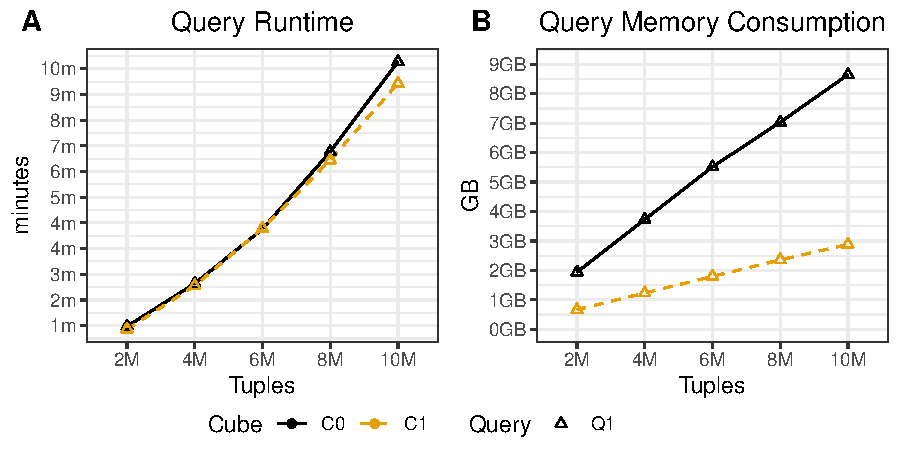
\includegraphics{Figuras/query1-1.pdf}}
  \end{center}
  \vspace{2mm}
  \legenda{(\textbf{A}) Total time to answer a query, including the time to read the data from the disk, build the cube and then answer the query Q1, with cubes C0 and C1. (\textbf{B}) Total memory consumption to answer Q1 with cubes C0 and C1.}
  \FONTE{Author.}
\end{figure}

\hypertarget{q2-1}{%
\subsubsection{Q2}\label{q2-1}}

Figure \ref{fig:query2}-A shows the query response times for query Q2, with the execution of the query in the C0 and C2 cubes.
Here the difference when \(\mathcal{T} =\ensuremath{10^{7}}\) is C2 having a runtime 40\% faster than C0.
Figure \ref{fig:query2}-B shows the query memory difference between C0 and C2 for query Q2.
Again the result is C2 taking only a fraction (14\%) of the same query under C0.

\begin{figure}[H]
  \caption{Query 2 results.}\label{fig:query2}
  \vspace{6mm}
  \begin{center}
    \resizebox{13cm}{!}{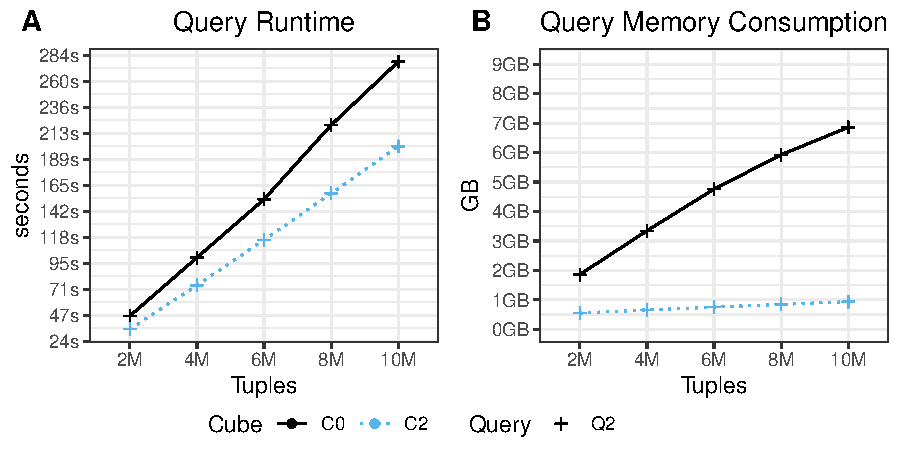
\includegraphics{Figuras/query2-1.pdf}}
  \end{center}
  \vspace{2mm}
  \legenda{(\textbf{A}) Total time to answer a query, including the time to read the data from the disk, build the cube and then answer the query Q2, with cubes C0 and C2. (\textbf{B}) Total memory consumption to answer Q2 with cubes C0 and C2.}
  \FONTE{Author.}
\end{figure}

\hypertarget{q3-1}{%
\subsubsection{Q3}\label{q3-1}}

Figure \ref{fig:query3}-A shows the query response times for query Q3, with the execution of the query in the C0 and C3 cubes.
With less inquires and dimensions this operation is expected to be faster, however the speedup is even greater: Q3 under C3 takes only 12\% of the memory used by C0.
Figure \ref{fig:query3}-B shows the query memory difference between C0 and C3 for query Q3, with C3 needing only 7\% of the memory used by C0.

\begin{figure}[H]
  \caption{Query 3 results.}\label{fig:query3}
  \vspace{6mm}
  \begin{center}
    \resizebox{13cm}{!}{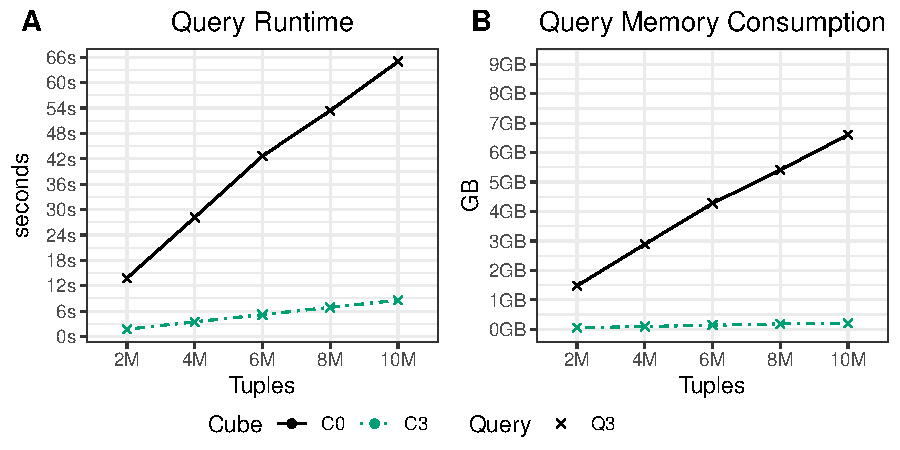
\includegraphics{Figuras/query3-1.pdf}}
  \end{center}
  \vspace{2mm}
  \legenda{(\textbf{A}) Total time to answer a query, including the time to read the data from the disk, build the cube and then answer the query Q3, with cubes C0 and C3. (\textbf{B}) Total memory consumption to answer Q3 with cubes C0 and C3.}
  \FONTE{Author.}
\end{figure}

\hypertarget{q4-1}{%
\subsubsection{Q4}\label{q4-1}}

Figure \ref{fig:query4}-A shows the query response times for query Q4, with the execution of the query in the C0 and C4 cubes.
Another query with only two dimensions, and expected to be faster, with C4 taking 5\% of the time used by C0.
Figure \ref{fig:query4}-B shows the query memory difference between C0 and C4 for query Q4, showing the same speedup pattern.

\begin{figure}[H]
  \caption{Query 4 results.}\label{fig:query4}
  \vspace{6mm}
  \begin{center}
    \resizebox{13cm}{!}{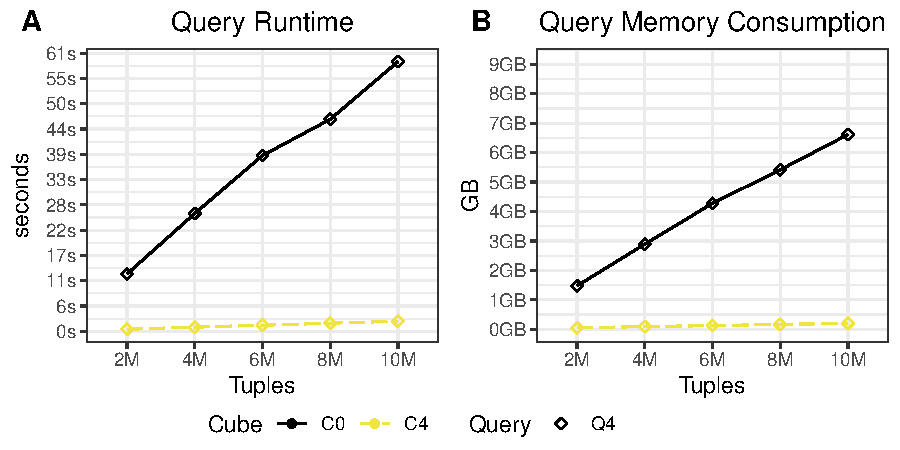
\includegraphics{Figuras/query4-1.pdf}}
  \end{center}
  \vspace{2mm}
  \legenda{(\textbf{A}) Total time to answer a query, including the time to read the data from the disk, build the cube and then answer the query Q4, with cubes C0 and C4. (\textbf{B}) Total memory consumption to answer Q4 with cubes C0 and C4.}
  \FONTE{Author.}
\end{figure}

\hypertarget{q5-1}{%
\subsubsection{Q5}\label{q5-1}}

Figure \ref{fig:query5}-A shows the query response times for query Q5, with the execution of the query in the C0 and C5 cubes.
Here with more dimensions than the previous two queries the speedup is less, but still substantial, with C5 taking only 43\% of the runtime used by C0.
Figure \ref{fig:query5}-B shows the query memory difference between C0 and C5 for query Q5, where the same figure of speedups are maintained.

\begin{figure}[H]
  \caption{Query 5 results.}\label{fig:query5}
  \vspace{6mm}
  \begin{center}
    \resizebox{13cm}{!}{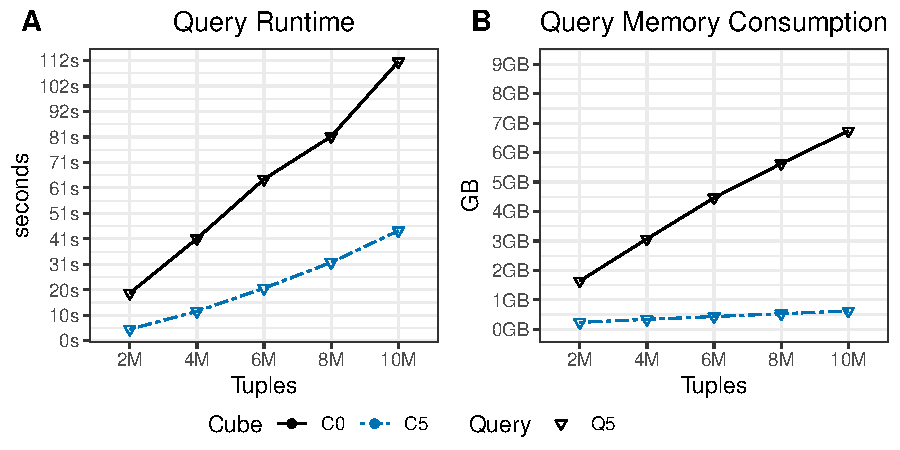
\includegraphics{Figuras/query5-1.pdf}}
  \end{center}
  \vspace{2mm}
  \legenda{(\textbf{A}) Total time to answer a query, including the time to read the data from the disk, build the cube and then answer the query Q5, with cubes C0 and C5. (\textbf{B}) Total memory consumption to answer Q5 with cubes C0 and C5.}
  \FONTE{Author.}
\end{figure}

\section{Summary and analysis}\label{ch:querypart:summary}

For this experiment, the time dimension has the property of having a cardinality that is approximately equal to the amount of tuples (\(\mathcal{C}_d = \mathcal{T}\), for a cardinality of dimension \(d\) and with a database of \(\mathcal{T}\) tuples), as each observation is time-stamped and therefore unique.
This creates a considerable skew to the results with all telemetries, as with \(\ensuremath{10^{7}}\) tuples, a single dimension with \(\mathcal{C}_d = {10}^7\) is not suitable to be computed entirely, and very different from the other dimensions that have a maximum cardinality of \(\mathcal{C}_d = 256\).
As this time dimension was not considered in any query, this is expected to have been one of the reasons for the great difference in memory consumption between the queries and $C0$.

In summary, these results show that building the cube with only the dimensions for a given query can yield up to 80 times less memory for the cube construction, and using between 1\% to 33\% less memory to answer the same query on the same data, with variations depending on the amount of inquired dimensions.
The speedup is so apparent that it'd be \emph{faster} to read, build and then answer a query using one of the low-dimensional cubes (\(C1-5\)) than to directly query an already built data cube with all dimensions (\(C0\)), and is the main contribution of this work.
Furthermore, the shell fragment size parameter shows little benefit in reducing the memory consumption of the queries when they are performed in this manner, and should be kept at 1.

It is also important to highlight the query definitions with the help of a domain expert: most queries are low dimensional in nature, in line with Frag-Cubing's strengths.
These queries are non-exhaustible and meant to be samples, but show that the common algorithmic approaches are suitable for the domain and can be made to improve memory implementation requirements.


%%%%%%%%%%%%%%%%%%%%%%%%%%%%%%%%%%%%%%%%%%%%%%%%%%%%%%%%%%%%%%%%%%%%%%%%%%%%%%%

\chapter{INTERVALFRAG}\label{ch:interval}

This section describes the IntervalFrag algorithm, and the proposed architecture needed to implement the enhancements to the Frag-Cubing's algorithm.

\section{Using Intervals in Inverted Indexes}\label{ch:interval:problem}

In chapter~\ref{ch:corr:cube:frag} the Frag-Cubing algorithm was explained, as per the original implementation by~\citeonline{liHighdimensionalOLAPMinimal2004}.
One of the key parts of the algorithm is the use of an inverted index to query directly into the attribute values and allow for the iceberg pruning of cells that fall below minimum support.
The algorithm depends on the intersection of TID lists to work, as that is how it can know what tuples have that specific value and where to find them to compute the relevant measures.
This part of the algorithm is mentioned by the original work as being done naively, and the original authors suggest some ways of compressing the index and speeding up the intersection of the lists, as this will be one of the most frequent operations that the algorithms needs to do to answer queries, and a speedup on this part would greatly enhance performance.

Furthermore, as most of the data is directly loaded into memory, using some form of compression on the inverted index would also reduce memory implementation requirements, and hopefully also query response times.
One of the strategies that they mention is by compressing the TID list into \textit{d-gaps}, in which each element is encoded by being the sum of the current element plus the previous element.
In general, for a list of numbers $\langle d_1, d_2 , \cdots, d_k \rangle$, the \textit{d-gap} list would be $\langle d_1 , d_2 - d_1 , \cdots, d_k - d_{k - 1} \rangle$.
The compression then would come from encoding the elements into a smaller number of bits, hopefully much less than the standard of 32 for an integer.
This approach takes advantage of the ordered nature of the TID list, as it is encoded from the tuples as they read and thus are naturally sorted non-zero positive integers.

This approach requires heavily changing the binary operations of the inverted index, however it is not the only one: since publication there are various different techniques to compress an inverted index, and they are an active branch of research.
More options, and a more complex implementation of the above method can be found into Elias-Fano encoding and the others mentioned in~\citeonline{pibiriTechniquesInvertedIndex2019}.
However, most of them require the use of dictionaries or heavy bit-encoding to achieve better results, which in general sacrifices the update operation.

One much simpler technique that has not been explored is the use of intervals instead of raw numbers in the TID list.
The inverted index structure is then kept, but each TID list now instead of containing the ordered numbers, contains an ordered list of intervals between each element.
For a list of numbers $\langle d_1, d_2 , \cdots, d_k \rangle$, the interval list would be $\langle [d_1, d_2] , [d_3, d_4], \cdots, [d_k, d_{k + 1}] \rangle$, where $d_k < d_{k+1}$, and the difference between the intervals cannot be smaller than one, thus $d_{k+1} - d_k \geq 1$.
Example: for the TID list $\langle 1, 3, 4, 5, 7 \rangle$, the Interval List would be $\langle [1, 1], [3, 5], [7, 7] \rangle$, where we can represent $3$ and $7$ that have no difference between their intervals as the singles $\langle [1], [3-5], [7] \rangle$.

This has implications only for the intersection of the lists, and is overall a much simpler implementation to execute.
By previous experience with the data, it was found that a great number of dimensions have attribute values that are repeated on long sequences of the same telemetry data points, and Frag-Cubing generates a long list of these repetitions for some dimensions.
This work then seeks to answer the question: \textbf{Can the use of the Interval algorithm instead of the raw list reduce memory requirements and query response times for long sequences of real world satellite telemetry data?}

Thus, in this chapter this implementation will be detailed, as well as an experiment to evaluate whether there is any advantage to using these intervals over the standard technique used by Frag-Cubing.

\section{Algorithm}\label{ch:interval:algo}

In practice, the algorithm cannot be implemented using two integers for each interval, as in the case where there is not a substantial interval (difference bigger than one) all elements will take the space of two integers when in Frag-Cubing they would take the place of only one integer.
This would lead to the worst case for the Interval algorithm to be double the memory of Frag-Cubing, but this can be worked around in practice by encoding the elements without an interval in the negative range of the integer, which isn't used in the TID list as each element indicates a unique identifier that is positive.

In case the identifier to be inserted would be close to zero, it is necessary to add one to each of the elements in the TID list as they are inserted into the IntervalIndex, as checking for a negative zero is not recommended and not guaranteed to work the same on every computer architecture \cite{ieeeIEEEStandardFloatingPoint2019}.
With this, the entire integer bit space is used, including the signal bit for the algorithm.
For the scope of this work, and since the experiment does not require the update of cells, only the insertion and intersection algorithms will be detailed.

Furthermore, it is necessary to define the concept of sequentiality, as it quantifies how much a list can be compressed by transforming it into a list of intervals.
A high sequentiality means that the data are repeated in long sequences, for example $\langle 1, 2, 3, 4, 5, 6, 7, 8, 9 \rangle$ can be compressed into the sequences $\langle [1, 9] \rangle$, being of high sequentiality.
However, the list $\langle 1, 3, 5, 6, 9\rangle$ would have a low sequentiality, as the resulting list interval would be only $\langle [1], [3], [5, 6], [9] \rangle$, and would consume exactly as much space as the raw list, with the conversion to an interval list being unfavorable.

\subsection{IntervalInsertion}\label{ch:interval:algo:insertion}

Insertions to the index can be done always by appending to the current list, as the TID are read in sequence and are naturally ordered positive integers.
Supposed that we're inserting an element $b$ to the list.
The insertion can be done by checking if the last element in the list is positive, if it is, then there is an interval and it is necessary to check the penultimate element in the list.
If the last element is negative $c$, then we can check if $c * -1 + 1 = b$, and if it is we flip the signal of the position $c$ and insert $b$ to the list as it is.
If the last element is not negative, then we check if the element $c$, is $c + 1 = b$ and update the position $c$ if it is true, else we flip the signal of $b$ and insert it at the end of the list.
Else none of these we can safely append $b$ to the end of the list after flipping the signal to negative, and thus this algorithm is implemented at $\Theta(1)$, shown in \autoref{algo:interval_insertion}.

\begin{algorithm}[!htb]
\SetAlgoLined
\KwResult{Element inserted into the list}
 $b$ element to be inserted\;
 $L$ the interval list to be inserted\;
 \If{$empty(L)$}{
   AppendList($L$, $b * - 1$)\;
   \KwRet\;
 }
 $c$ = LastElement($L$)\;
 \eIf{$c < 0$}{
   \If{$c * -1 + 1 = b$}{
     $L[c] = L[c] * - 1$ \tcp*{Update the last to be positive}
     AppendList($L$, $b$)\;
     \KwRet\;
   }
 }{
   \If{$b + 1 = c$}{
     $L[c] = b$ \tcp*{Update last element}
     \KwRet\;
   }
 }
 AppendList($L$, $b * - 1$) \tcp*{None of the previous cases, just append the element as a negative}
 \caption{IntervalInsertion}\label{algo:interval_insertion}
\end{algorithm}

\subsection{IntervalIntersection}\label{ch:interval:algo:intersection}

The problem of intersecting two sets of elements is a big one, and will not be fully explored by this work, however a simple exploration of some algorithms that was a byproduct of this work are available in Appendix~\ref{ap:a:problem}.
However, due to the change in how the index uses the TID list, it is necessary to adapt the Frag-Cubing set intersection algorithm to still calculate the intersection between two intervals, and so the IntervalIntersection algorithm is created.

In order to check if two intervals intersect: assuming two intervals $I_a = \langle a_l, a_r \rangle$ and $I_b = \langle b_l, b_r \rangle$, where $a_l$ is the smallest element in the interval, and $a_r$ the biggest element in the interval.
The output intersection can be defined as $I_o = \langle a_l, a_r \rangle$, and the intersection $I_o = I_a \bigcap I_b$ can be computed by computing the biggest element between $a_r$ and $b_r$ (function $max$) and the smallest element between $a_l$ and $b_l$ (function $min$), or \autoref{algo:intersect_interval}.

\begin{algorithm}[!htb]
\SetAlgoLined
\KwResult{The result intersection $I_o$, or $\emptyset$ in case there is no intersection}
 $I_a$ and $I_b$ two intervals\;
  \eIf{$b_l > a_r$ or $a_l > b_l$}{
    \KwRet $\emptyset$\;
  }{
  $o_l$ = $max( a_l, b_l )$\;
  $o_r$ = $min( a_r, b_r )$\;
  \KwRet $[o_l, o_r]$\;
  }
  \caption{IntersectTwoIntervals, adapted from \cite{26260}}\label{algo:intersect_interval}
\end{algorithm}

\autoref{fig:interval:sample} shows four examples of using this algorithm to select for intersections, including the empty case when there is no intersection.
For the list interval intersection, it can be naively implemented using the scalar merge strategy: two pointers walk by each interval, check if there is an intersection between then and, if there is, create a new element in the result list with the intersection between these two intervals.
The algorithm to perform this is shown below, and takes the same complexity of the parent algorithm of $\mathcal{O}(n + m)$, where $n$ and $m$ are the sizes of the interval lists being intersected.
This resulting algorithm is based on the implementations by \citeonline{liHighdimensionalOLAPMinimal2004} and \citeonline{silva:2015:abordagensParaCubo}, shown in \autoref{algo:intersect_interval_lists}.

\begin{figure}[!htb]
  \caption{IntervalIntersection example}\label{fig:interval:sample}
  \vspace{6mm}
  \begin{center}
    \resizebox{9cm}{!}{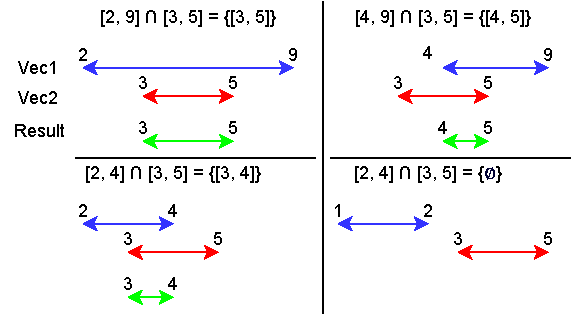
\includegraphics{Figuras/IntervalIntersection-Cases.pdf}}
  \end{center}
  \vspace{2mm}
  \legenda{IntervalIntersection example with four operations}
  \FONTE{Author}
\end{figure}

\begin{algorithm}[H]
\SetAlgoLined
\KwResult{The resulting list intersection between two interval lists, or $\emptyset$ if there is no intersection}
 $L_a$ and $L_b$ two input interval lists\;
 $L_c$ result list, with maximum size $min(length(L_a), length(L_b))$\;
 $a_i, b_i, c_i = 0$\;
 \While{$a_i < length(L_a)$ and $b_i < length(L_b)$}{
   $A[a_l, a_r]$ = interval($L_a[a_i$]) \tcp*{Gets the interval at this position}
   $B[b_l, b_r]$ = interval($L_b[a_i$])\;
  \If{$b_l \leq a_r$ and $a_l \leq b_r$}{
    IntervalInsertion($L_c$, IntersectTwoIntervals(A, B)) \tcp*{Insert into the result list the intersection between the elements}
    NextIntervalPosition($c_i$) \tcp*{Skips to the next available list space}
  }
  \eIf{$a_r \leq b_r$}{
   NextIntervalPosition($a_i$)\;
   }{
   NextIntervalPosition($b_i$)\;
  }
 }
 \KwRet{$L_c$}\;
 \caption{IntervalIntersection}\label{algo:intersect_interval_lists}
\end{algorithm}

\section{Results}\label{ch:interval:results}

\autoref{tab:interval_memory} and~\autoref{tab:interval_query} show the results of executing both algorithms to answer the queries defined in \autoref{ch:querypart:queries}, while using the cube structure defined as $C0$ in \autoref{ch:querypart:exp:method}, where all telemetries were used as a single file for each test, and then the query was executed, measuring the memory consumption in the first and query response time in the latter.

\begin{table}[!ht]
  \centering
  \caption{IntervalFrag x Frag-Cubing, memory consumption in KiB}\label{tab:interval_memory}
  \begin{tabular}{|c|c|c|c|c|c|c|c|}
    \hline
    & & \multicolumn{5}{c|}{\textbf{Tuples}} \\
    \hline
    \bfseries Algorithm & \bfseries Query & \bfseries $2\times10^6$ & \bfseries $4\times10^6$ & \bfseries $6\times10^6$ & \bfseries $8\times10^6$ & \bfseries $1\times10^7$\\
    \hline
    \multirow{5}{*}{Frag-Cubing} & Q1 &
    1.908.708 & 3.674.784 & 5.447.864 & 6.953.424 & 8.557.348
    \\\cline{2-7} & Q2 &
    1.842.396 & 3.294.628 & 4.727.816 & 5.877.016 & 6.760.080
    \\\cline{2-7} & Q3 &
    1.448.280 & 2.836.592 & 4.236.496 & 5.362.128 & 6.502.628
    \\\cline{2-7} & Q4 &
    1.444.816 & 2.836.696 & 4.236.404 & 5.372.104 & 6.520.176
    \\\cline{2-7} & Q5 &
    1.607.456 & 3.024.996 & 4.445.800 & 5.591.052 & 6.650.456
    \\\hline
    \multirow{5}{*}{IntervalFrag} & Q1 &
    504.428 & 845.804 & 1.196.504 & 1.455.472 & 1.651.552
    \\\cline{2-7}
    & Q2 &
    801.864 & 1.207.760 & 1.560.652 & 1.752.292 & 2.062.560
    \\\cline{2-7} & Q3 &
    388.652 & 707.588 & 1.030.392 & 1.237.324 & 1.415.472
    \\\cline{2-7}
    & Q4 &
    370.624 & 690.456 & 1.003.236 & 1.237.292 & 1.415.456
    \\\cline{2-7}
    & Q5 &
    540.788 & 895.272 & 1.232.520 & 1.412.280 & 1.604.288
    \\\hline
  \end{tabular}
\end{table}

\begin{table}[!ht]
  \centering
  \caption{IntervalFrag x Frag-Cubing, query response times in ms}\label{tab:interval_query}
  \begin{tabular}{|c|c|c|c|c|c|c|c|}
    \hline
    & & \multicolumn{5}{c|}{\textbf{Tuples}} \\
    \hline
    \bfseries Algorithm & \bfseries Query & \bfseries $2\times10^6$ & \bfseries $4\times10^6$ & \bfseries $6\times10^6$ & \bfseries $8\times10^6$ & \bfseries $1\times10^7$\\
    \hline
    \multirow{5}{*}{Frag-Cubing} & Q1 &
    5.4691 & 188.634 & 310.455 & 421.409 & 523.772
    \\\cline{2-7} & Q2 &
    47.391 & 108.405 & 170.515 & 258.585 & 281.877
    \\\cline{2-7} & Q3 &
    1.557 & 3.089 & 4.637 & 6.497 & 7.597
    \\\cline{2-7} & Q4 &
    399 & 817 & 1.193 & 1.573 & 1.990
    \\\cline{2-7} & Q5 &
    7.138 & 21.668 & 33.483 & 49.590 & 59.428
    \\\hline
    \multirow{5}{*}{IntervalFrag} & Q1 &
    1.946 & 4.712 & 6.981 & 9.198 & 11.508
    \\\cline{2-7}
    & Q2 &
    158.050 & 333.838 & 554.111 & 772.125 & 934.793
    \\\cline{2-7} & Q3 &
    3.570 & 7.064 & 10.655 & 14.812 & 17.714
    \\\cline{2-7}
    & Q4 &
    995 & 2.011 & 2.952 & 3.860 & 4.916
    \\\cline{2-7}
    & Q5 &
    4.871 & 11.837 & 18.477 & 26.176 & 32.649
    \\\hline
  \end{tabular}
\end{table}

In order to make the comparisons easier to understand, let's focus on only queries $Q1$ and $Q2$, that were the highest number of dimensions and the highest number of cardinalities respectively.
\autoref{fig:interval:q1-2} shows those results, and it is clear that the memory usage is always much lower under IntervalFrag.
$Q1$ has four dimensions with low cardinality and high sequentiality, and these are quickly answered by IntervalFrag, while Frag-Cubing takes a long time to answer the queries that involve those dimensions.

However, in the case of $Q2$ where all dimensions have both cardinality and low sequentiality, IntervalFrag takes 331\% longer to answer the query on the worst case, being the biggest drawback of this algorithm.
This is due to the inherently slower set intersection algorithm used by IntervalFrag, that needs to execute more comparisons than Frag-Cubing, even when the algorithms have the same complexity and are similar.

\begin{figure}[H]
  \caption{IntervalFrag for Q1 and Q2}\label{fig:interval:q1-2}
  \vspace{6mm}
  \begin{center}
    \resizebox{13cm}{!}{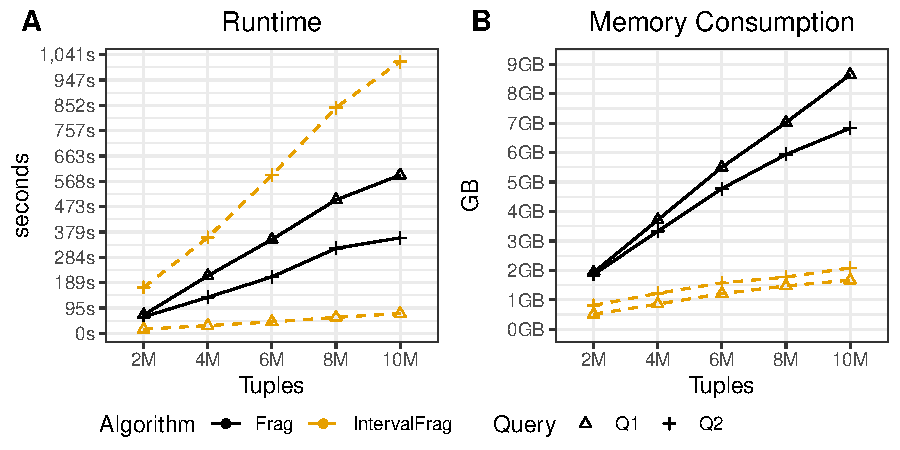
\includegraphics{Figuras/q1q2-1.pdf}}
  \end{center}
  \vspace{2mm}
  \legenda{
    (\textbf{A}) Query response times of IntervalFrag and Frag-Cubing for queries $Q1$ and $Q2$ under the cube $C0$
    (\textbf{B}) Memory consumption of IntervalFrag and Frag-Cubing for queries $Q1$ and $Q2$ under the cube $C0$.
}
  \FONTE{Author}
\end{figure}

In the case of queries $Q3$, $Q4$ and $Q5$, IntervalFrag is slower to answer queries $Q3$ and $Q4$, both that have a high cardinality and low sequentiality, but takes only about 53\% of the time to answer $Q5$, that also has a high cardinality but presents a high sequentiality.
\autoref{fig:interval:q3-4} shows those results for $Q3$ and $Q4$, \autoref{fig:interval:q5} for $Q5$, and it is also clear that the memory usage is much lower with IntervalFrag than with Frag-Cubing.

\begin{figure}[H]
  \caption{IntervalFrag for Q3 and Q4}\label{fig:interval:q3-4}
  \vspace{6mm}
  \begin{center}
    \resizebox{13cm}{!}{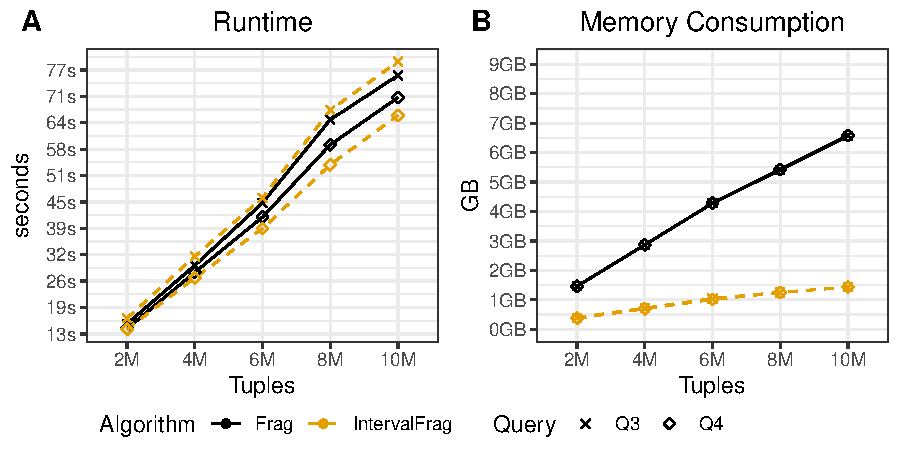
\includegraphics{Figuras/q3q4-1.pdf}}
  \end{center}
  \vspace{2mm}
  \legenda{
    (\textbf{A}) Query response times of IntervalFrag and Frag-Cubing for queries $Q3$ and $Q4$ under the cube $C0$
    (\textbf{B}) Memory consumption of IntervalFrag and Frag-Cubing for queries $Q3$ and $Q4$ under the cube $C0$.
}
  \FONTE{Author}
\end{figure}

\begin{figure}[H]
  \caption{IntervalFrag for Q5}\label{fig:interval:q5}
  \vspace{6mm}
  \begin{center}
    \resizebox{13cm}{!}{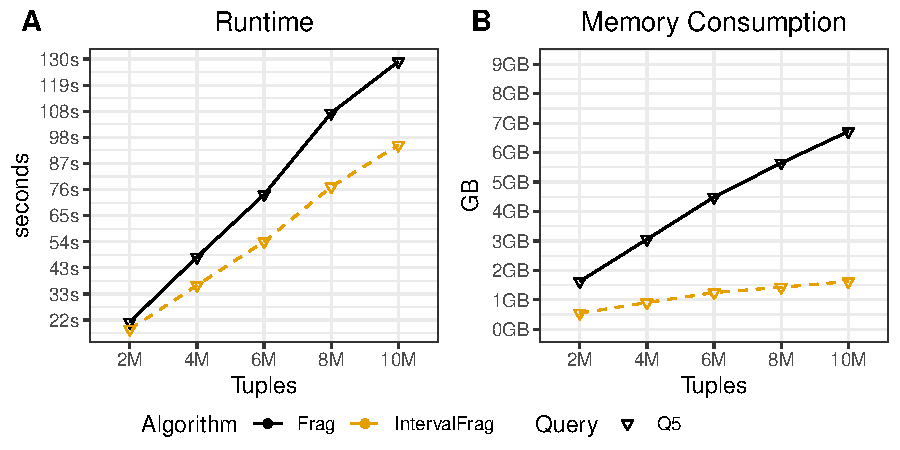
\includegraphics{Figuras/q5-1.pdf}}
  \end{center}
  \vspace{2mm}
  \legenda{
    (\textbf{A}) Query response times of IntervalFrag and Frag-Cubing for queries $Q5$ under the cube $C0$
    (\textbf{B}) Memory consumption of IntervalFrag and Frag-Cubing for queries $Q5$ under the cube $C0$.
}
  \FONTE{Author}
\end{figure}

Additionally, we need to compare the time necessary to create the cube under each of the algorithms, here called Time to Cube.
If one algorithm takes too long to transverse the cube structure and execute the minimum support pruning this would need to be counted against it, however as~\autoref{fig:interval:timetocube} shows, the difference between IntervalFrag and Frag-Cubing is not that big, with IntervalFrag being on average 10\% slower than Frag-Cubing.
This however is just a simple comparison, as in that step each subcube of the fragments would be computed and for these tests that use $\mathcal{F} = 1$ they are almost exactly the same computation, needing higher fragment sizes to appreciate the difference.
However, since this computation would involve list intersections at higher fragment sizes, the speed of the intersection algorithm would heavily influence this computation, being more comparable to the query response times compared above.

\begin{figure}[H]
  \caption{Comparison: Time to Cube}\label{fig:interval:timetocube}
  \vspace{6mm}
  \begin{center}
    \resizebox{13cm}{!}{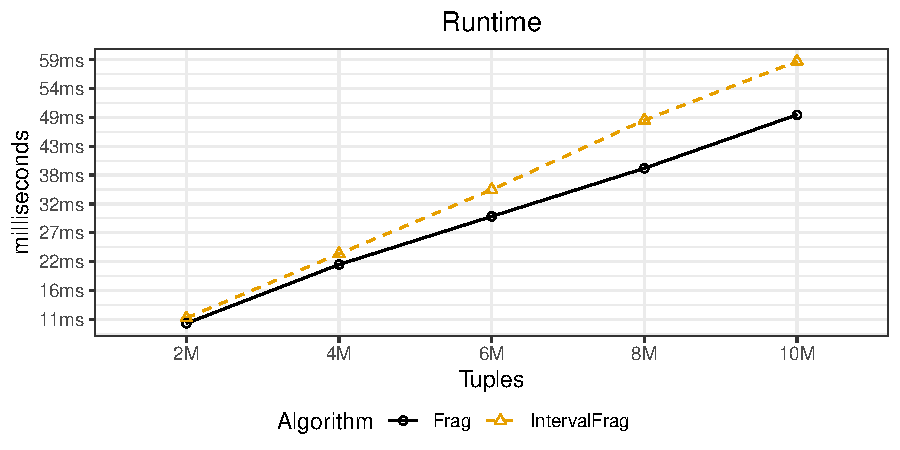
\includegraphics{Figuras/timetocube-1.pdf}}
  \end{center}
  \vspace{2mm}
  \legenda{Time necessary to compute the cube after the data is read into memory.}
  \FONTE{Author}
\end{figure}

Another important metric is the baseline memory used before queries can be performed on the data.
\autoref{fig:interval:baseline} shows these values for the files used in this experiment, and IntervalFrag consumes on average 22\% of the memory that Frag-Cubing needs.
This is important as it allows IntervalFrag to be implemented while requiring much less computational resources.

\begin{figure}[H]
  \caption{Comparison: Baseline memory}\label{fig:interval:baseline}
  \vspace{6mm}
  \begin{center}
    \resizebox{13cm}{!}{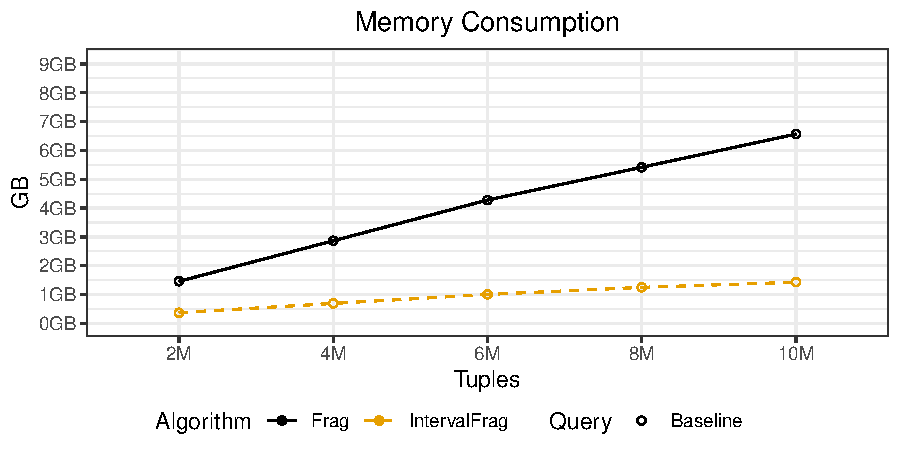
\includegraphics{Figuras/baseline-1.pdf}}
  \end{center}
  \vspace{2mm}
  \legenda{Memory used by the baseline cube, when it can start to answer queries}
  \FONTE{Author}
\end{figure}

\section{Summary}\label{ch:interval:summary}

FragInterval was up to 3 times slower to answer queries on dimensions with low sequentiality and high cardinality, but was faster to answer queries on dimensions with high sequentiality.
On all queries FragInterval used only between 20\% and 24\% of the memory that Frag-Cubing used, being the biggest improvement that IntervalFrag brings.
Furthermore, FragInterval also needed only on average 22\% of the memory that Frag-Cubing used to compute the baseline cube, before the queries can be answered, while being only 10\% slower to compute.

Thus, FragInterval shows to be preferred on environments with low available RAM, as long as the slower queries with higher cardinalities are acceptable.
FragInterval achieves the objective of answering the queries with much less memory, however fails at having comparable response times than Frag-Cubing on high dimensionality queries.
This slowness is due to the set intersection algorithm in IntervalFrag having to execute more comparisons in practice than Frag-Cubing's, and thus being slower when the sets have the same size and the data has low sequentiality to favor IntervalFrag's algorithm.


%%%%%%%%%%%%%%%%%%%%%%%%%%%%%%%%%%%%%%%%%%%%%%%%%%%%%%%%%%%%%%%%%%%%%%%%%%%%%%%

\chapter{Analysis and Discussion}\label{ch:analysis}

In this chapter, a critical analysis of the algorithms is presented, as well as an overview of how useful are the results and what are their shortcomings.
The results from chapters~\ref{ch:interval} and~\ref{ch:querypart} show that simple approaches can be used to enhance the query response time for the selected queries, and can be easily ported to other domains and styles of computation.

\autoref{tab:analysis_overview} shows the characteristics in which each algorithm has showed to excel at.
Frag-Cubing is still preferred when the data has a low degree of sequentiality, as there's little advantage in using the IntervalFrag scheme when the intervals are closer to the size of the original list.
On those cases, IntervalFrag is discouraged, as the algorithm will be slower than Frag-Cubing's by simple virtue of needing more instructions to answer the same query, being up to 400\% slower than the same query under Frag-Cubing.

\begin{table}[!ht]
  \centering
  \caption{Preferred algorithm to use}\label{tab:analysis_overview}
  \footnotesize
  \begin{tabular}{|C{1.8cm}|C{2.3cm}|C{2.3cm}|C{2.65cm}|C{2cm}|C{1.6cm}|}
    \hline
    & \bfseries Low Sequentiality &\bfseries High Sequentiality &\bfseries High Dimensionality &\bfseries High Cardinality &\bfseries High Skew \\
    \hline
    Computing the base cube & IntervalFrag & IntervalFrag & IntervalFrag & IntervalFrag& IntervalFrag \\
    \hline
    Subcube query & Frag-Cubing & IntervalFrag & IntervalFrag & Frag-Cubing$^1$ & FragCubing \\
    \hline
    Point query & Frag-Cubing & IntervalFrag & IntervalFrag & Frag-Cubing$^1$ & FragCubing \\
    \hline
    Low available RAM & IntervalFrag & IntervalFrag & IntervalFrag & IntervalFrag & IntervalFrag \\
    \hline
    Fast Query Reponse & Frag-Cubing & IntervalFrag & Frag-Cubing$^1$ & Frag-Cubing$^1$ & Frag-Cubing \\
    \hline
    \multicolumn{6}{l}{$^{1}$\footnotesize{If there's high sequentiality, prefer IntervalFrag}} \\
  \end{tabular}
\end{table}
\normalsize

In summary, in case the RAM available is low and the worst case query response times can be up to 4x slower than Frag-Cubing's, then IntervalFrag should be preferred as the main method of computing the data cube.
In case the data have a very low sequentiality, and RAM is available, then using Frag-Cubing should still be preferred for the faster response times.
IntervalFrag will excel at any dimension that has a high sequentiality, even if it also has a high cardinality, however dimensions that have a high cardinality will tend to have a low sequentiality in practice, and this usage might be rarer.
The Skew parameter can influence the algorithm both ways, as it does not necessarily mean that the dimension will have a higher or lower sequentiality and cardinalities.

When the dimensions have a high degree of sequentiality, then IntervalFrag excels, as it can not only answer the same queries much faster, but also using only a fraction of the memory used by Frag-Cubing.
Furthermore, Frag-Cubing used much less memory to answer queries $Q1$, $Q2$ and $Q5$, with $Q4$ having a small difference and $Q3$ having no difference in memory usage in the end, when compared with cubes $C1$ to $C5$.
All queries executed on the $C0$ cube with all dimensions used only a fraction of the memory needed to answer queries with IntervalFrag, they were however in general slower to answer.

From the tests made using Frag-Cubing and the different cubes ($C1$ to $C5$) tailored to specific queries, it was shown that the best algorithms can be further enhanced by doing some simple pre-processing of the queries, and depending on the type of query used they can drastically improve upon memory usage requirements, allowing for some frequent queries to be optimized and even allowing for queries that could not be answered under a $C0$ cube to be answered by smaller cubes.
In chapter~\ref{ch:querypart} it was shown that it is faster to load a smaller subset of the data in memory as prepared files when needed and then computing the answer from that file instead of querying a cube that was already loaded in memory, but that used the full dimensional capability of the data.

\RED{ADD AT LEAST ONE GRAPH OR TABLE COMPARING THEM. THE ONE USED FOR THE PRESENTATION IS FINE}

It is important to note IntervalFrag had faster file reading speeds (about 12\% faster) due to improvements made on the implementation, as well as a slightly more efficient set intersection algorithm, which were not backported to Frag-Cubing.
This was done to preserve the Frag-Cubing algorithm's performance, as the original code was made for the C language in 2002 and the updated IntervalFrag implementation uses C++17 standards.
Nonetheless, it was possible to compile Frag-Cubing using the same flags as IntervalFrag under the GNU C++ compiler, with minimal performance differences.

The difference in query response times from IntervalFrag and Frag-Cubing, even when using the same intersection algorithm, was due to IntervalFrag having to do more comparisons to answer the same query, and this implementation could not be further optimized without heavily skewing the response times to IntervalFrag's side, by using other techniques that could also be ported to Frag-Cubing trivially.
Further details on the intersection algorithms tested and their performance differences can be found on Appendix~\ref{ap:a:problem}.


%%%%%%%%%%%%%%%%%%%%%%%%%%%%%%%%%%%%%%%%%%%%%%%%%%%%%%%%%%%%%%%%%%%%%%%%%%%%%%%

\chapter{CONCLUSIONS}\label{ch:concl}

This work shows that it is possible to further optimize data cube algorithms by gathering information from the underlying data, and how this can be made to aid the end user's experience by decreasing implementation requirements and improving response times.

\section{Main contributions}\label{ch:concl:contrib}

One of the stated purposes of this work was to find ways of using the data's domain characteristics to improve the satellite operator's day to day activities, and this work has achieved three main results:

\begin{enumerate}
\item A heuristic to discover related telemetries between satellite time series data and how to use this with the help of an operator to validate the relevant queries;
\item Using the previous heuristic to enhance Frag-Cubing's query response time and memory by pre-partitioning the data;
\item Improving upon Frag-Cubing's Inverted Index memory model by saving only intervals instead of the entire values, and thus reducing memory and query response times for some queries;
\end{enumerate}

\RED{This is still all wrong. What do?}

\section{Future work}\label{ch:concl:future}

The natural evolution of this work would be to test it using other data cube algorithms, as there's a great variety of them mentioned in section~\ref{ch:corr} and not all of them might be applicable to satellite telemetry data, or showcase useful performance metrics.
On that note the use of bCubing~\cite{silva:2015:abordagensParaCubo} will be interesting, as the inverted index separation into blocks can further improve upon the memory usage as described in this chapter.

The use of the gathered satellite data on other projects is also of interest, as there's no public reliable dataset of satellite telemetry data that contains all relevant data and not just a subset of a subsystem, and this work showcases a volume that has information enough for the training of Machine Learning and Artificial Intelligence projects.
Only projects that release full telemetry data are relatively simple CubeSat projects, who do not generate a significant volume that is enough for the use of these algorithms.
The author plans to release the dataset in a citable format for the use of the community in the near future.

This work also has the potential of improving query execution when dealing with multiple satellites, constellations and/or formations, it needing only the data to be gathered and the suitable cube format defined to be tested.

The relationship algorithms mentioned in~\autoref{ch:querypart:heur} can be remade to use other different solutions, and combined with the shell-cubing method to generate only shells that have relationships above a certain strength.
This was also one of the ideas to be developed during this work, which however had not enough time to be fully developed.
This idea is best when paired with known "best available" techniques, like using the project ~\cite{LibrespacefoundationPolarisPolaris2021}.

Furthermore the Set Intersection problem defined in chapter~\ref{ch:interval} can be further optimized with recent advances not only in computer architectures, but also with regards to complexity and the validation of the algorithms in real world datasets.
A preliminary investigation was performed, as a simple but not rigorous overview of the results is detailed in Appendix~\ref{ap:a}.

\section{Final thoughts}\label{ch:concl:future}

\RED{The approach and architecture detailed in this work...}

This work was developed entirely with open source software, and they will be made available later at \url{https://github.com/Yuri-M-Dias/SCD2}.
Furthermore, there is a lack of good datasets that deal with satellite telemetry data available, perhaps this work can further contribute by allowing the usage of the dataset by making it public.
The volume available here is much bigger than what is currently used by Machine Learning competitions, and the publication can further enhance work in this area.



%% insira quantos capítulos desejar com o seguinte comando:
%\include{_pasta_do_arquivo_/_meu_arquivo_} %%sem a extensão
%% note que deverá haver um arquivo _meu_arquivo_.tex (com extensão) no diretório _pasta_do_arquivo_

%\include{./docs/conclusao}

%% Bibliografia %% não alterar %% obrigatório %testebib
\bibliography{./bib/EXAM} %% aponte para seu arquivo de bibliografia no formato bibtex (p.ex: referencia.bib)

%\include{./docs/glossario} %% insira os termos do glossário no arquivo glossario.tex %% opcional

\inicioApendice %% opcional, comente esta linha e a seguintes se não houver apendice(s)
%%%%%%%%%%%%%%%%%%%%%%%%%%%%%%%%%%%%%%%%%%%%%%%%%%%%%%%
%Apêndice A
\hypertarget{estilo:apendice1}{} %% uso para este Guia
%Este apêndice foi criado apenas para indicar como construir um apêndice no estilo, não existia no original da tese.
%%%%%%%%%%%%%%%%%%%%%%%%%%%%%%%%%%%%%%%%%%%%%%%%%%%%%%
\renewcommand{\thechapter}{}%
\chapter{APÊNDICE A - AUTORIZAÇÃO PARA PUBLICAÇÃO}	% trocar A por B na próxima apêndice e etc
\label{apendiceA}	% trocar A por B na próxima apêndice e etc
\renewcommand{\thechapter}{A}%		% trocar A por B na próxima apêndice e etc

Há dois formulários de autorização para publicação, um para publicações de trabalhos acadêmicos e outro para publicações técnico-científicas, neste apêndice encontram-se os modelos dos formulários e suas respectivas instruções de preenchimento. 

\section{Autorização para Publicação de Trabalho Acadêmico - INPE-393}

\label{instr393}

	\begin{figure}[ht]
		\caption{Formulário Autorização para Publicação de Trabalho Acadêmico INPE-393.}
		\vspace{6mm}	% acrescentar o espaçamento vertical apropriado entre o título e a borda superior da figura
		\centering
   		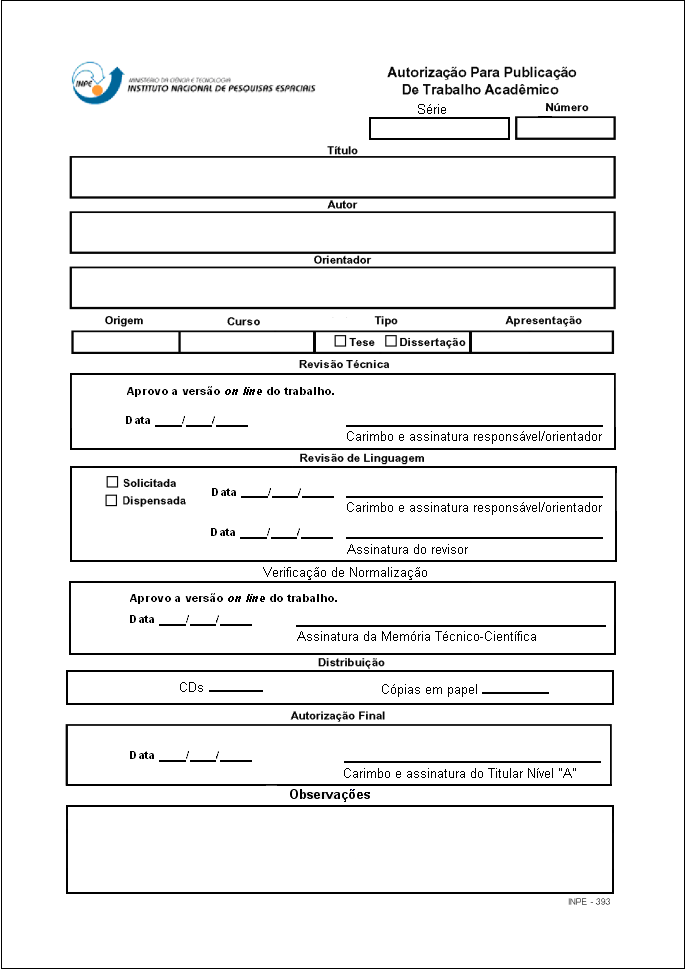
\includegraphics[height=16cm]{./Figuras/form393.png}	   
 		\label{form393}
	\end{figure}


\subsection{Instruções do Formulário INPE-393} 

\begin{enumerate} 

 \item \textbf{série:} com este número o SID identifica as publicações do INPE, composto da sigla da Instituição, número sequencial geral da publicação, sigla e número sequencial do tipo de publicação, exemplo: INPE-14209-TDI/1110;
 
 \item \textbf{número:} será composto da sigla da unidade do SID, mais 4 (quatro) dígitos e do ano em curso. Este número de referência é de controle da unidade emissora. Ex.: SID-0001/2007;

 \item \textbf{título da publicação:} deve ser completo, evitando-se abreviar palavras;

 \item \textbf{nome do autor e do orientador:} estes campos devem ser preenchidos por extenso, da mesma forma em que irão constar da publicação;

 \item \textbf{origem da publicação:} sigla da unidade do servidor (autor da publicação), conforme TQ-001;

 \item \textbf{curso:} sigla do curso, de acordo com a Estrutura de Divisão de Trabalho - EDT do INPE;
 
 \item \textbf{tipo:} assinalar se é tese ou dissertação;

 \item \textbf{apresentação:} colocar a data de aprovação final;

 \item \textbf{revisão técnica:} o responsável designado pela Banca Examinadora para verificação de correções e, na ausência desse, o orientador da tese ou dissertação deve
carimbar, datar e assinar após a versão \emph{on line} do trabalho;

 \item \textbf{revisão de linguagem:} o responsável designado pela Banca Examinadora para verificação de correções, e na ausência deste o orientador deve assinalar a solicitação ou a dispensa da revisão de linguagem e, carimbar, datar e assinar; o revisor deve datar e assinar após a revisão;
 
 \item \textbf{distribuição:} O SID deve informar a quantidade de CD's e de cópias impressas da tese ou dissertação, conforme lista de distribuição;
 
 \item \textbf{verificação de normalização:}  Após a verificação da versão \emph{on line} do trabalho quanto às normas editoriais, o SID deve datar e assinar;
 
 \item \textbf{autorização final:} data e assinatura do Titular de Nível A, conforme TQ-001, a que o Serviço de Pós-Graduação estiver subordinado.
 
 \item \textbf{observações:} para outras informações necessárias. 

\end{enumerate}

\section{Autorização para Publicação - INPE-106}
\begin{figure}[ht!]
	\caption{Formulário Autorização para Publicação de Trabalho Acadêmico INPE-106 folha 1.} 
	\vspace{6mm}	% acrescentar o espaçamento vertical apropriado entre o título e a borda superior da figura
	\centering
	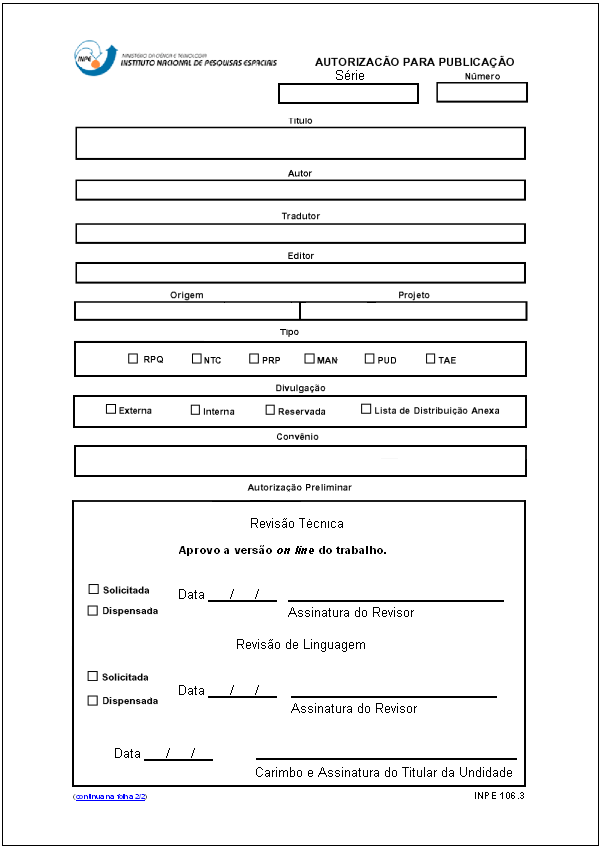
\includegraphics[height=18cm]{./Figuras/form106.png}
	\label{form106}
\end{figure}

\begin{figure}[ht!]
	\caption{Formulário Autorização para Publicação de Trabalho Acadêmico INPE-106 folha 2.} 
	\vspace{6mm}	% acrescentar o espaçamento vertical apropriado entre o título e a borda superior da figura
	\centering
	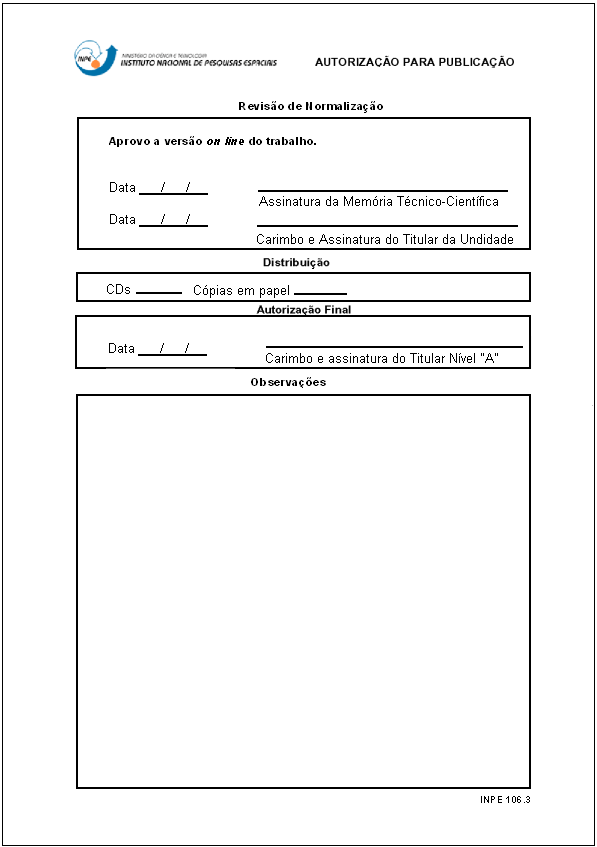
\includegraphics[height=18cm]{./Figuras/form106folha2.png}
	\label{form106a}
\end{figure}

\clearpage
\subsection{Instruções do Formulário INPE-106} 
\label{instr106}


\begin{enumerate}

 \item \textbf{série:} com este número o SID identifica as publicações do INPE, composto da sigla da Instituição, número sequencial geral da publicação, sigla e número sequencial do tipo de publicação, exemplo: INPE-5616-RPQ/671. 
 
 \item \textbf{número:} será composto da sigla da unidade constante da Estrutura Organizacional do INPE (TQ-001), mais 4 (quatro) dígitos e do ano em curso. Este número de referência é de controle da unidade solicitante. Ex: CEA-0001/2007;
 
 \item \textbf{título da publicação:} deve ser completo, evitando-se abreviar palavras;

 \item \textbf{nome do autor, tradutor e editor:}  estes campos devem ser preenchidos por extenso, da mesma forma em que irão constar da publicação;

 \item \textbf{origem da publicação:} sigla da unidade do servidor (autor da publicação), conforme TQ-001;

 \item \textbf{projeto:} sigla do projeto de acordo com a Estrutura de Divisão de Trabalho - EDT do INPE;

 \item \textbf{tipo de publicação:} assinalar o tipo de publicação proposta:

 \begin{enumerate}
  \item{Relátorio de Pesquisa (RPQ)},
  \item{Notas Técnico-Científicas (NTC)},
  \item{Propostas e Relatórios de de Projeto (PRP)},
  \item{Manuais Técnicos (MAN)},
  \item{Publicações Didáticas (PUD)},
  \item{Trabalhos Acadêmicos Externos (TAE)}.
 \end{enumerate}

 \item \textbf{divulgação:} assinalar, de acordo com os critérios de classificação. Se houver Lista de Divulgação, nesta deverá constar os nomes e endereços completos;

 \item \textbf{convênio:} descrever o nome da instituição, quando a publicação for realizada pelo INPE e outra organização, preencher somente para o tipo PRP; 
 
    \item \textbf{autorização preliminar:} data, carimbo e assinatura do Titular da Unidade a que o autor esteja subordinado e, assinatura do revisor que efetuou a revisão técnica aprovando a versão \emph{on line} do trabalho e do revisor que realizou a revisão de linguagem, quando solicitadas; 
    
  \item \textbf{verificação de normalização:} o SID deve datar e assinar após a revisão da adequação às normas editoriais;   
  
  \item \textbf{distribuição:} O SID deve informar a quantidade de CD's e de cópias impressas que deverão ser gravados conforme lista de distribuição;
  
 \item \textbf{autorização final:} data, carimbo e assinatura do Titular de Nível "A", conforme TQ-001, a que o autor da publicação estiver subordinado;
 
 \item \textbf{observações:} para outras informações necessárias, inclusive para descrever as justificativas de uma publicação.
\end{enumerate} %% insira apendices tal qual capítulos acima
%%%%%%%%%%%%%%%%%%%%%%%%%%%%%%%%%%%%%%%%%%%%%%%%%%%%%%%%%%%%%%%%%%%%%%%%%%%%%%%%%

\hypertarget{appendix:a}{} %% uso para este Guia
\renewcommand{\thechapter}{}%
\chapter{APPENDIX A - INTERSECTION ALGORITHMS}
\label{ap:a}
\renewcommand{\thechapter}{A}

\section{Problem}\label{ap:a:problem}

This is only a simple overview to show the importance of the problem and how different algorithms stack against each other.

The problem can be stated as follows: given sets $S_1$ and $S_2$, find the elements that are present in both sets, their intersection, represented as $S_1 \cap S_2$.
Furthermore, each element is ordered as unique, for they represented index positions and are thus always non-zero positive integers.

\section{Algorithms}\label{ap:a:algos}

\textcolor{red}{All wrong for now}

UnorderedSet

Scalar

Li

BinaryLi

std::set\_intersect

SIMD (SS2)


\section{Experiments}\label{ap:a:results}

To search for the best algorithm with real world data, an experiment was performed, much on the same framework as detailed in~\ref{ch:querypart:exp:method}: C++ code, each test was executed 5 times and the median of the values was taken.
As each technique is efficient with the memory usage, there wasn't much difference to be measured, so only the time necessary to intersect each list was measured.
Each list was generated in interval from $2\times10^6$ to $1\times10^7$, and all algorithms work on randomized ordered lists with the same size.
This spread was intentional to mirror the worst cases in the Frag-Cubing algorithm.

Table~\ref{tab:setresults} showcases a summary of the experiment's results, this time caring only for the necessary time to answer the queries.

\begin{table}[!ht]
  \begin{center}
    \caption{Set Intersection Results, in milliseconds}\label{tab:setresults}
    \begin{tabular}{|c|c|c|c|c|c|c|}
      \hline
      \textbf{Algorithm - N} & \bfseries $2\times10^6$ & \bfseries $4\times10^6$ & \bfseries $6\times10^6$ & \bfseries $8\times10^6$ & \bfseries $1\times10^7$\\
      \hline
      UnorderedSet & 867,802 & 1806,19 & 2586,04 & 3448,11 & 4213,15\\
      \hline
      Scalar & 26,57 & 51,346 & 71,109 & 85,531 & 118,114\\
      \hline
      Li & 26,531 & 45,596 & 66,19 & 86,234 & 108,603\\
      \hline
      BinaryLi & 21,601 & 39,776 & 59,27 & 79,416 & 97,155\\
      \hline
      std::set\_intersect & 17,125 & 34,392 & 51,682 & 67,717 & 84,933\\
      \hline
      SIMD (SS2) & 10,941 & 21,854 & 33,866 & 43,739 & 55,814\\
      \hline
    \end{tabular}
  \end{center}
\end{table}

As the HashSet approach was the slowest approach, \autoref{fig:set_intersection_results} showcases the comparison between the other algorithms, that have comparable performances and are easier to visualize.

\begin{figure}[ht]
  \caption{Set Intersection Algorithm results}\label{fig:set_intersection_results}
  \vspace{6mm}
  \begin{center}
    \resizebox{12cm}{!}{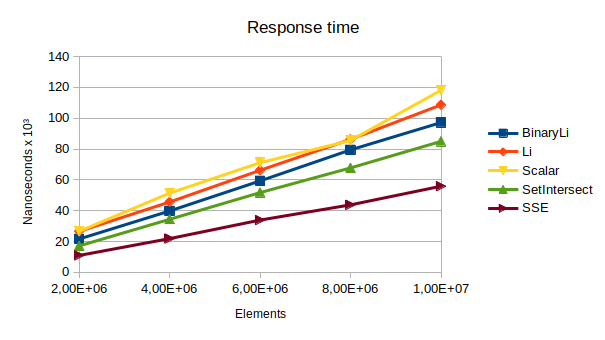
\includegraphics{Figuras/IndexListResult.png}}
  \end{center}
  \vspace{2mm}
  \legenda{Set intersection algorithms response times in milliseconds, ordered by the size of the input relation.}
  \FONTE{Author}
\end{figure}

The SIMD approach is clearly the fastest, however it is also dependant on processor architecture and even though the used SIMD instructions (SS2) are available on almost all modern CPUs, other newer instruction sets might not be, or might have different implementations depending on the CPU vendor, which complicates widespread implementation.

While these tests are interesting, there was not enough time to test some recent benchmarks that found the use of different algorithms and could improve the performance of each, as the use of compressed indexes in \cite{pibiriTechniquesInvertedIndex2019} show.
Furthermore, the SIMD instruction set used here (SSE2) is limited even if it's support is widespread, with other instruction sets (SSE3, AVX, AVX512, etc) being available on modern CPUs and also available for use.

Some recent results that have not been properly explored in the data cube context as of yet: Recursive Universe Partitioning, a technique that uses the possible search space to partition the sets and execute the intersection~\cite{pibiriFastCompactSet2021}; FESIA, which combines the use of previous techniques with different SIMD computation techniques and a bitmap to decide which algorithm is more suitable for use depending on the set size~\cite{zhangFESIAFastSIMDEfficient2020}; and simpler implementations that reduce branch mispredictions~\cite{inoueFasterSetIntersection2014}, and the use of pre-processed dictionaries to greatly aid in the computation~\cite{dingFastSetIntersection2011a}.
There's even an algorithm to compute the set intersection in $\mathcal{O}(1)$ by using a quantum computer~\cite{tianQuantumAlgorithmFinding2019}, however that approach is likely not implementable for any significant dataset in the near future.

Further testing is necessary when dealing with lists of varying sizes, that would showcase the improvements of certain algorithms over others, and the incorporation of these algorithms into a real-world dataset for accurate tests.



\inicioAnexo
%%%%%%%%%%%%%%%%%%%%%%%%%%%%%%%%%%%%%%%%%%%%%%%%%%%%%%%%%%%%%%%%%%%%%%%%%%%%%%%%%

\renewcommand{\thechapter}{}%
\chapter{ANEXO A - CRONOGRAMA}
\label{anexoA}
\renewcommand{\thechapter}{A}

\begin{table}[!ht]
  \label{tab:cronograma}
  \begin{center}
	\caption{Cronograma de atividades}
	\begin{tabular*}{\textwidth}{|p{3cm}|c|c|c|c|c|c|c|c|c|c|} %%11!
		\hline
		\textbf{Atividade} & maio & jun. & jul. & ago. & set. & out. & nov. & dec. & jan. & fev. \\
		\hline
		Entrevista de qualificação &X&&&&&&&&& \\
		\hline
		Submissão Artigo Periódico &&&&&X&&&&& \\
		\hline
		Apresentação Conferência &&&&&&X&&&& \\
		\hline
		Defesa final &&&&&&&X&&&X \\
		\hline
	\end{tabular*}
   \end{center}
\end{table}



\inicioIndice
%%%%%%%%%%%%%%%%%%%%%%%%%%%%%%%%%%%%%%%%%%%%%%%%%%%%%%
%Contracapa
%%%%%%%%%%%%%%%%%%%%%%%%%%%%%%%%%%%%%%%%%%%%%%%%%%%%%%

\thispagestyle{empty}
 \begin{table}
  \begin{center}
  \begin{tabularx}{\textwidth}{X}
   \textbf{PUBLICAÇÕES TÉCNICO-CIENTÍFICAS EDITADAS PELO INPE}
  \end{tabularx} 
  \end{center}
 \end{table}
  
 \begin{table}
  \begin{center}
  \begin{tabularx}{\textwidth}{X X}
      
  \textbf{Teses e Dissertações (TDI)}              & \textbf{Manuais Técnicos (MAN)}\\
\\
Teses e Dissertações apresentadas nos Cursos de Pós-Graduação do INPE.	&
São publicações de caráter técnico que incluem normas, procedimentos, instruções e orientações.\\
\\
\textbf{Notas Técnico-Científicas (NTC)}           & \textbf{Relatórios de Pesquisa (RPQ)}\\
\\
Incluem resultados preliminares de pesquisa, descrição de equipamentos, descrição e ou documentação de programas de computador, descrição de sistemas e experimentos, apresentação de testes, dados, atlas, e documentação de projetos de engenharia. 
&	
Reportam resultados ou progressos de pesquisas tanto de natureza técnica quanto científica, cujo nível seja compatível com o de uma publicação em periódico nacional ou internacional.\\
\\
\textbf{Propostas e Relatórios de Projetos (PRP)}	& \textbf{Publicações Didáticas (PUD)} 
\\
\\
São propostas de projetos técnico-científicos e relatórios de acompanhamento de projetos, atividades e convênios.
&	
Incluem apostilas, notas de aula e manuais didáticos. \\
\\         
\textbf{Publicações Seriadas} 	& \textbf{Programas de Computador (PDC)}\\
\\
São os seriados técnico-científicos: boletins, periódicos, anuários e anais de eventos (simpósios e congressos). Constam destas publicações o Internacional Standard Serial Number (ISSN), que é um código único e definitivo para identificação de títulos de seriados. 
&	
São a seqüência de instruções ou códigos, expressos em uma linguagem de programação compilada ou interpretada, a ser executada por um computador para alcançar um determinado objetivo. Aceitam-se tanto programas fonte quanto os executáveis.\\
\\
\textbf{Pré-publicações (PRE)} \\
\\
Todos os artigos publicados em  periódicos, anais e como capítulos de livros. \\                 \end{tabularx}
  \end{center}
 \end{table}



\end{document}
